\documentclass[11pt, a4paper]{article}

% --- 1. 页面与中文支持 ---
\usepackage[a4paper, top=2.5cm, bottom=2.5cm, left=2cm, right=2cm]{geometry}
\usepackage[UTF8]{ctex} % 中文支持

% --- 2. 功能宏包 ---
% [修正1] 去掉了 [draft] 选项,否则图片只会显示为空白框
\usepackage{graphicx}       
\usepackage{float}          % 强制图片位置 [H]
\usepackage{booktabs}       % 专业三线表
\usepackage{subcaption}     % 子图支持
\usepackage{enumitem}       % 列表格式定制
\usepackage{listings}       % 代码块支持
\usepackage{xcolor}         % 颜色支持
\usepackage{hyperref}       % 超链接
\usepackage{titlesec}
\usepackage{tocloft} % 控制目录格式

% --- 3. 样式详细设置 ---
\setlist[itemize]{label=-}
% 让页面底部不强行对齐,减少因浮动造成的空白页
\raggedbottom
% 缩小图与正文的间距
\setlength{\textfloatsep}{10pt}
\setlength{\intextsep}{10pt}

% 代码块设置
\definecolor{codegray}{rgb}{0.95,0.95,0.95}
\definecolor{keywordcolor}{rgb}{0.0, 0.0, 0.7}
\definecolor{commentcolor}{rgb}{0.0, 0.5, 0.0}

\lstset{
    backgroundcolor=\color{codegray},
    basicstyle=\ttfamily\small,
    breaklines=true,
    frame=single,
    columns=flexible,
    numbers=left,
    numberstyle=\tiny\color{gray},
    keywordstyle=\color{keywordcolor},
    commentstyle=\color{commentcolor},
    stringstyle=\color{purple},
    showstringspaces=false,
    extendedchars=false, 
    language=Python      
}

% [修正2] 注释掉了 graphicspath,改用显式路径以避免同名文件冲突
% \graphicspath{{./dataset/}{./Ncutresults/}{./cityscapes_result/}{./voc_results/}{./SAMresults-vit_b/}{./SAMresults-vit_h/}}

% 定义四级标题 subsubsubsection
\titleclass{\subsubsubsection}{straight}[\subsubsection]
\newcounter{subsubsubsection}[subsubsection]
\renewcommand\thesubsubsubsection{\thesubsubsection.\arabic{subsubsubsection}}
\titleformat{\subsubsubsection}[runin]
  {\normalfont\normalsize\bfseries}{\thesubsubsubsection}{1em}{}
\titlespacing*{\subsubsubsection}
  {0pt}{3.25ex plus 1ex minus .2ex}{1em}

% 设置目录深度为4级
\setcounter{tocdepth}{3}
\setcounter{secnumdepth}{3} % 设置章节编号深度为4级

% 自定义目录项格式,支持四级标题
\makeatletter
\newcommand*\l@subsubsubsection{\@dottedtocline{4}{7em}{4em}}
\makeatother

\begin{document}

% --- 封面页 ---
\begin{titlepage}
    \centering
    \vspace*{3cm}
    {\Huge \textbf{图像处理与计算机视觉研讨课:\\第二章作业} \par}
    \vspace{4cm}
    {\Large \textbf{姓名:} \underline{\makebox[5cm]{张宗桪}} \par}
    \vspace{1cm}
    {\Large \textbf{学号:} \underline{\makebox[5cm]{2023K8009991013}} \par}
    \vfill
    {\large \today \par}
    \vspace{2cm}
\end{titlepage}

% --- 目录页 ---
\newpage
\tableofcontents
\newpage

% --- 正文开始 ---

\section{环境配置 (Environment Setup)}

\subsection{SAM 模型配置}
SAM 的配置主要包括安装官方库以及下载不同规模的预训练权重(ViT-B 和 ViT-H)。

\begin{lstlisting}[language=bash, caption={SAM 环境安装与权重下载}]
# 1. 安装 segment-anything 库
pip install git+https://github.com/facebookresearch/segment-anything.git

# 2. 下载预训练权重文件
wget https://dl.fbaipublicfiles.com/segment_anything/sam_vit_h_4b8939.pth
wget https://dl.fbaipublicfiles.com/segment_anything/sam_vit_b_01ec64.pth
\end{lstlisting}

\begin{lstlisting}[language=Python, caption={SAM 模型加载代码示例}]
from segment_anything import sam_model_registry, SamPredictor

sam_checkpoint_h = "sam_vit_h_4b8939.pth"
model_type_h = "vit_h"
sam_h = sam_model_registry[model_type_h](checkpoint=sam_checkpoint_h)

sam_checkpoint_b = "sam_vit_b_01ec64.pth"
model_type_b = "vit_b"
sam_b = sam_model_registry[model_type_b](checkpoint=sam_checkpoint_b)
\end{lstlisting}

\subsection{DeepLab v3+ 模型使用}
下载Deeplab v3+ 在 Cityscapes 和 Pascal VOC 数据集上的预训练权重,并使用以下命令进行测试。

\begin{lstlisting}[language=Python, caption={DeepLab v3+ 模型测试脚本}]
# 使用 cityscapes
python predict.py --input dataset/4.jpg \
            --dataset cityscapes \
            --model deeplabv3plus_mobilenet \
            --ckpt checkpoints/best_deeplabv3plus_mobilenet_cityscapes_os16.pth \
            --save_val_results_to cityscapes_result

# 使用 pascal voc
python predict.py --input dataset/5.jpg \
            --dataset voc \
            --model deeplabv3plus_mobilenet \
            --ckpt checkpoints/best_deeplabv3plus_mobilenet_voc_os16.pth \
            --save_val_results_to voc_results
\end{lstlisting}

\subsection{归一化图割}
具体实现基于 \texttt{scikit-image} 库。

\begin{lstlisting}[language=Python, caption={基于 SLIC 超像素的归一化图割实现代码}]
from skimage import segmentation, color, graph
import cv2
import os

profile_dir = './dataset'
os.makedirs("./Ncutresults", exist_ok=True)

for file in os.listdir(profile_dir):
    image = cv2.imread(os.path.join(profile_dir, file))
    img = cv2.cvtColor(image, cv2.COLOR_BGR2RGB)
    labels1 = segmentation.slic(img, compactness=30, n_segments=200, start_label=1)
    g = graph.rag_mean_color(img, labels1, mode='similarity')
    labels2 = graph.cut_normalized(labels1, g)
    out2 = color.label2rgb(labels2, img, kind='avg', bg_label=0)
    out2_bgr = cv2.cvtColor((out2 * 255).astype('uint8'), cv2.COLOR_RGB2BGR)
    cv2.imwrite(os.path.join("./Ncutresults", f"ncut_{file}"), out2_bgr)
\end{lstlisting}

\newpage
\section{实验结果展示}
本章节展示归一化图割、DeepLab v3+ 以及 SAM 在公开数据集和自采数据集上的分割效果。

% --- 下面使用了显式路径 (Explicit Paths) 解决同名文件冲突 ---

\subsection{公开数据集测试结果}

% --- 测试用例 1 ---
\begin{figure}[htbp]
    \centering
    % 原图
    \begin{subfigure}{0.3\textwidth}
        \centering
        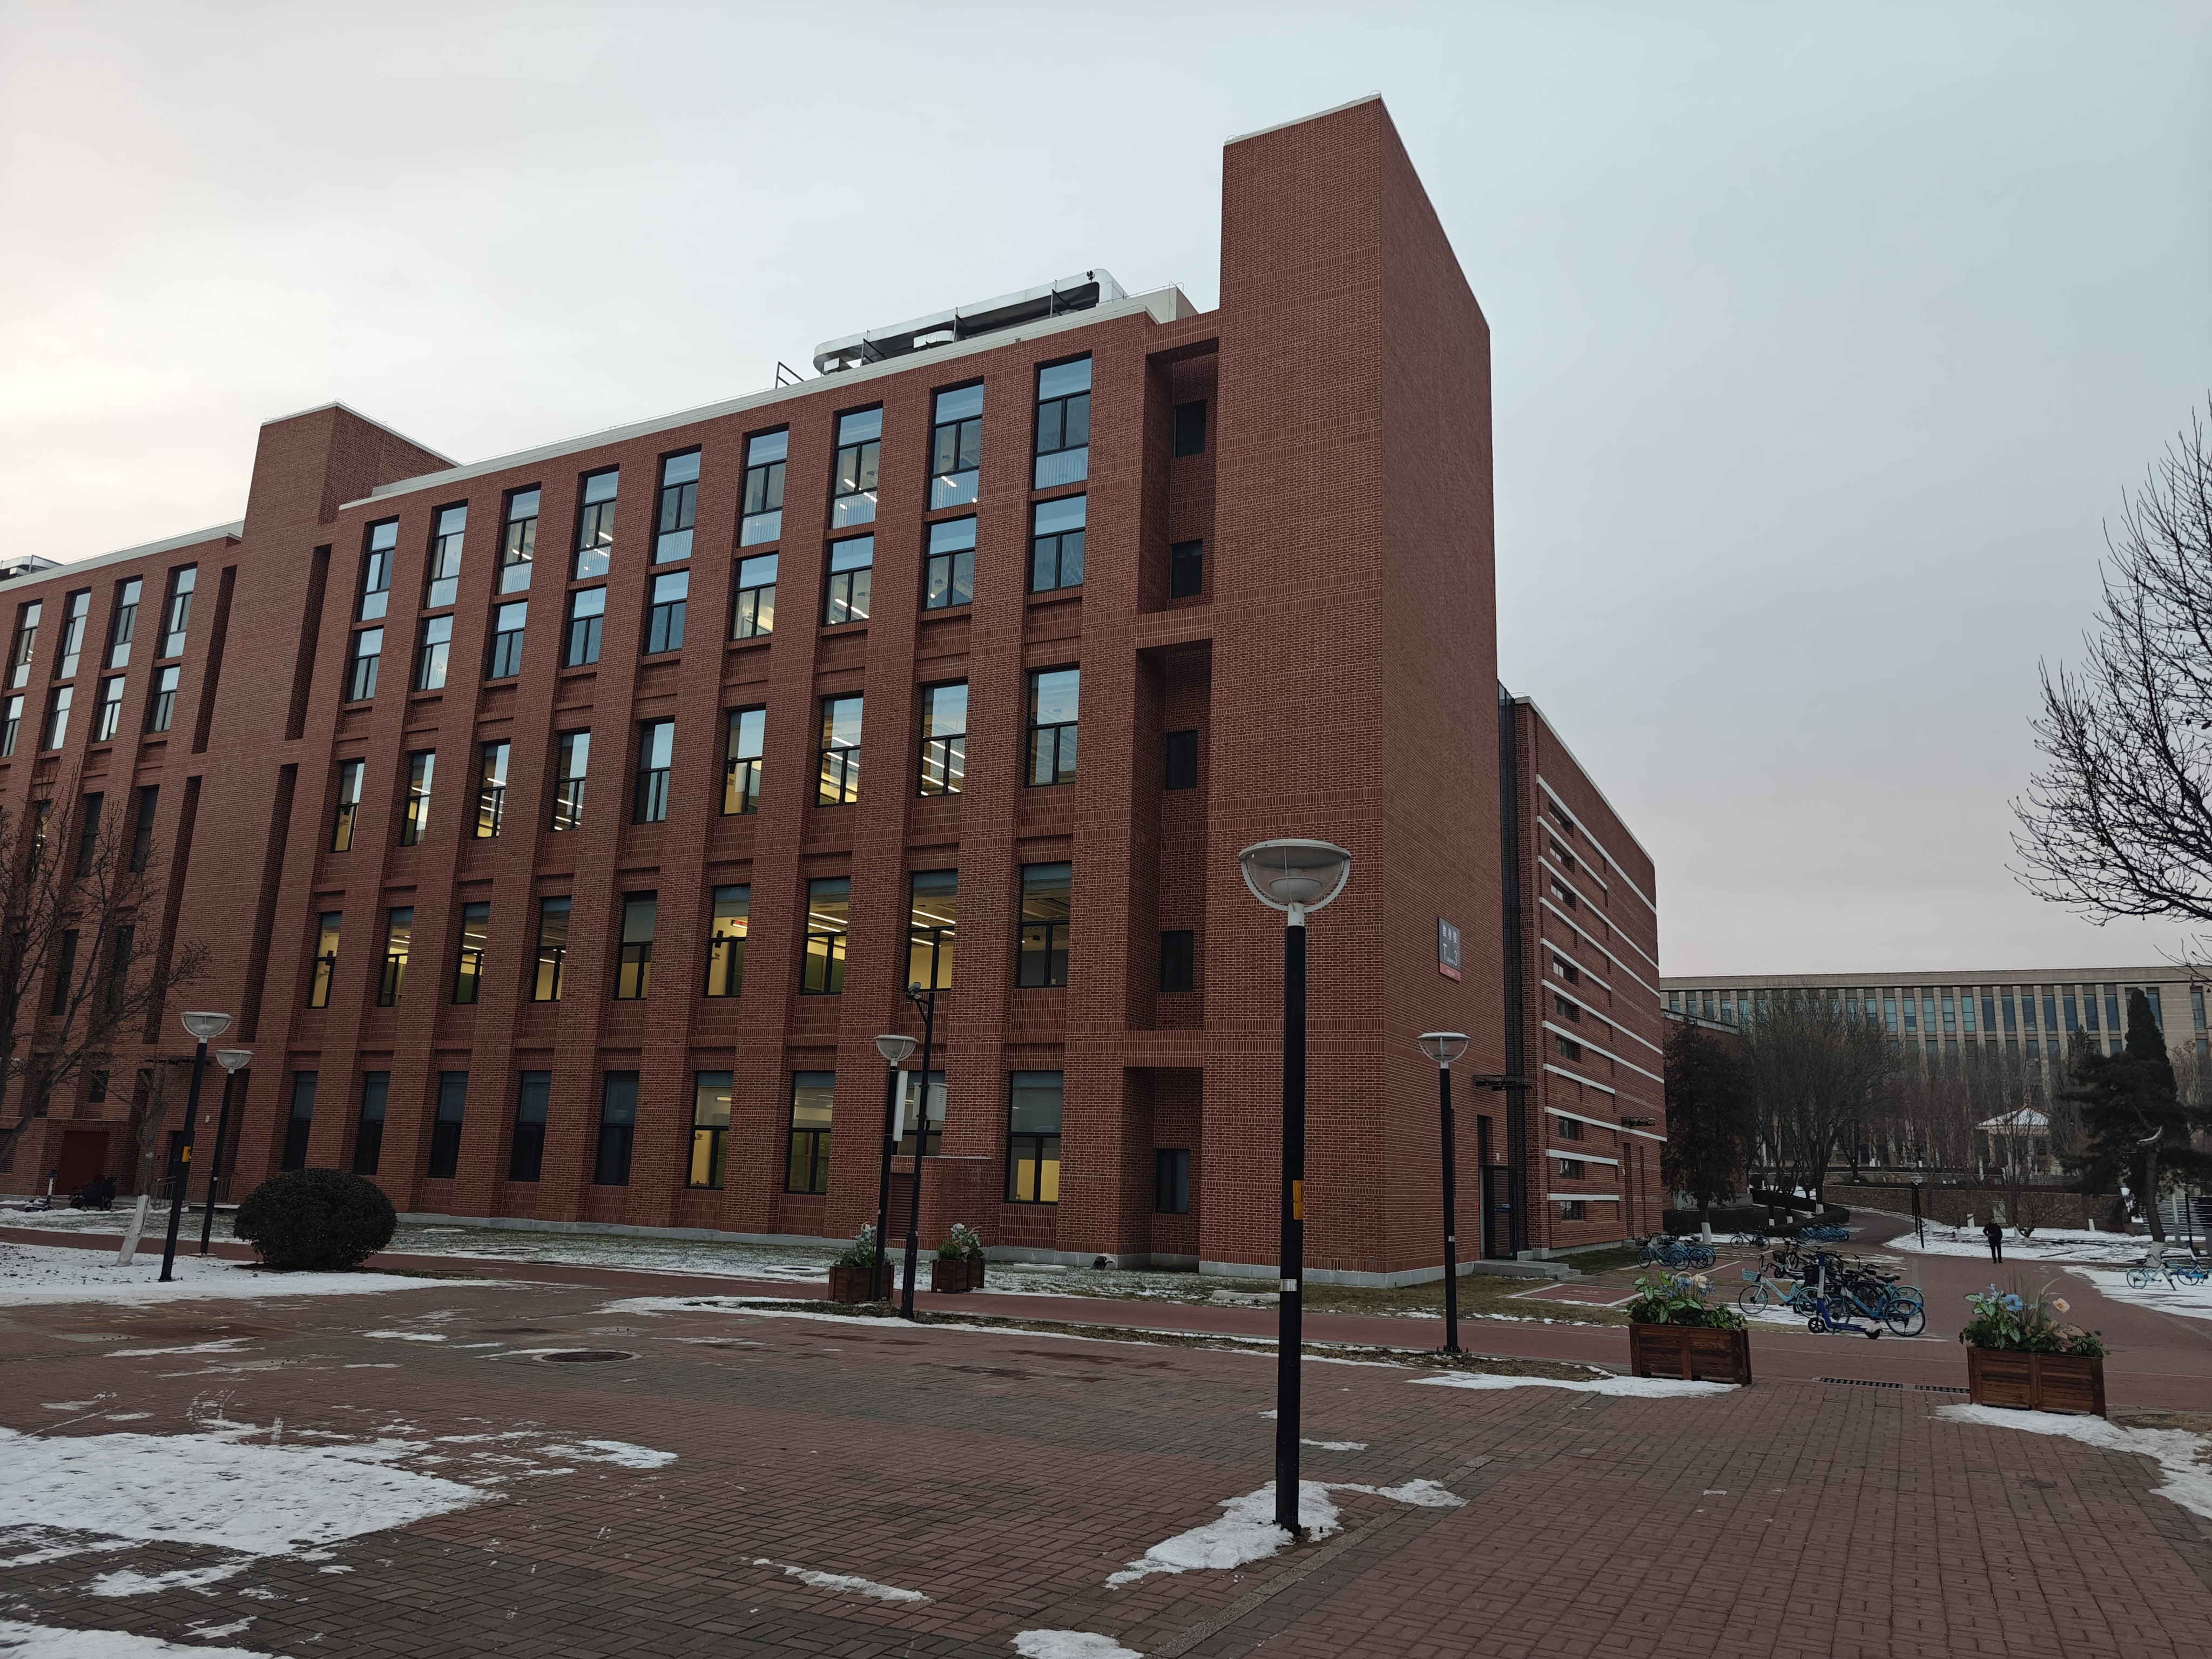
\includegraphics[width=\linewidth]{dataset/1.jpg} 
        \caption{原图 (Original)}
    \end{subfigure}
    \hfill
    % Ncut
    \begin{subfigure}{0.3\textwidth}
        \centering
        \includegraphics[width=\linewidth]{Ncutresults/ncut_1.jpg}
        \caption{Normalized Cuts}
    \end{subfigure}
    \hfill
    % Cityscapes
    \begin{subfigure}{0.3\textwidth}
        \centering
        \includegraphics[width=\linewidth]{cityscapes_result/1_semantic.png}
        \caption{DeepLab (Cityscapes)}
    \end{subfigure}
    
    \vspace{1em}
    
    % VOC (明确指定文件夹)
    \begin{subfigure}{0.3\textwidth}
        \centering
        \includegraphics[width=\linewidth]{voc_results/1semantic.png}
        \caption{DeepLab (Pascal VOC)}
    \end{subfigure}
    \hfill
    % SAM ViT-B (带下划线 sam_1)
    \begin{subfigure}{0.3\textwidth}
        \centering
        \includegraphics[width=\linewidth]{SAMresults-vit_b/sam_1.png}
        \caption{SAM (ViT-B)}
    \end{subfigure}
    \hfill
    % SAM ViT-H (注意:根据截图这里似乎没有下划线 sam1)
    \begin{subfigure}{0.3\textwidth}
        \centering
        \includegraphics[width=\linewidth]{SAMresults-vit_h/sam1.png}
        \caption{SAM (ViT-H)}
    \end{subfigure}
    
    \caption{公开数据集测试用例 1}
    \label{fig:public_case1}
\end{figure}

% --- 测试用例 2 ---
\begin{figure}[htbp]
    \centering
    \begin{subfigure}{0.3\textwidth}
        \centering
        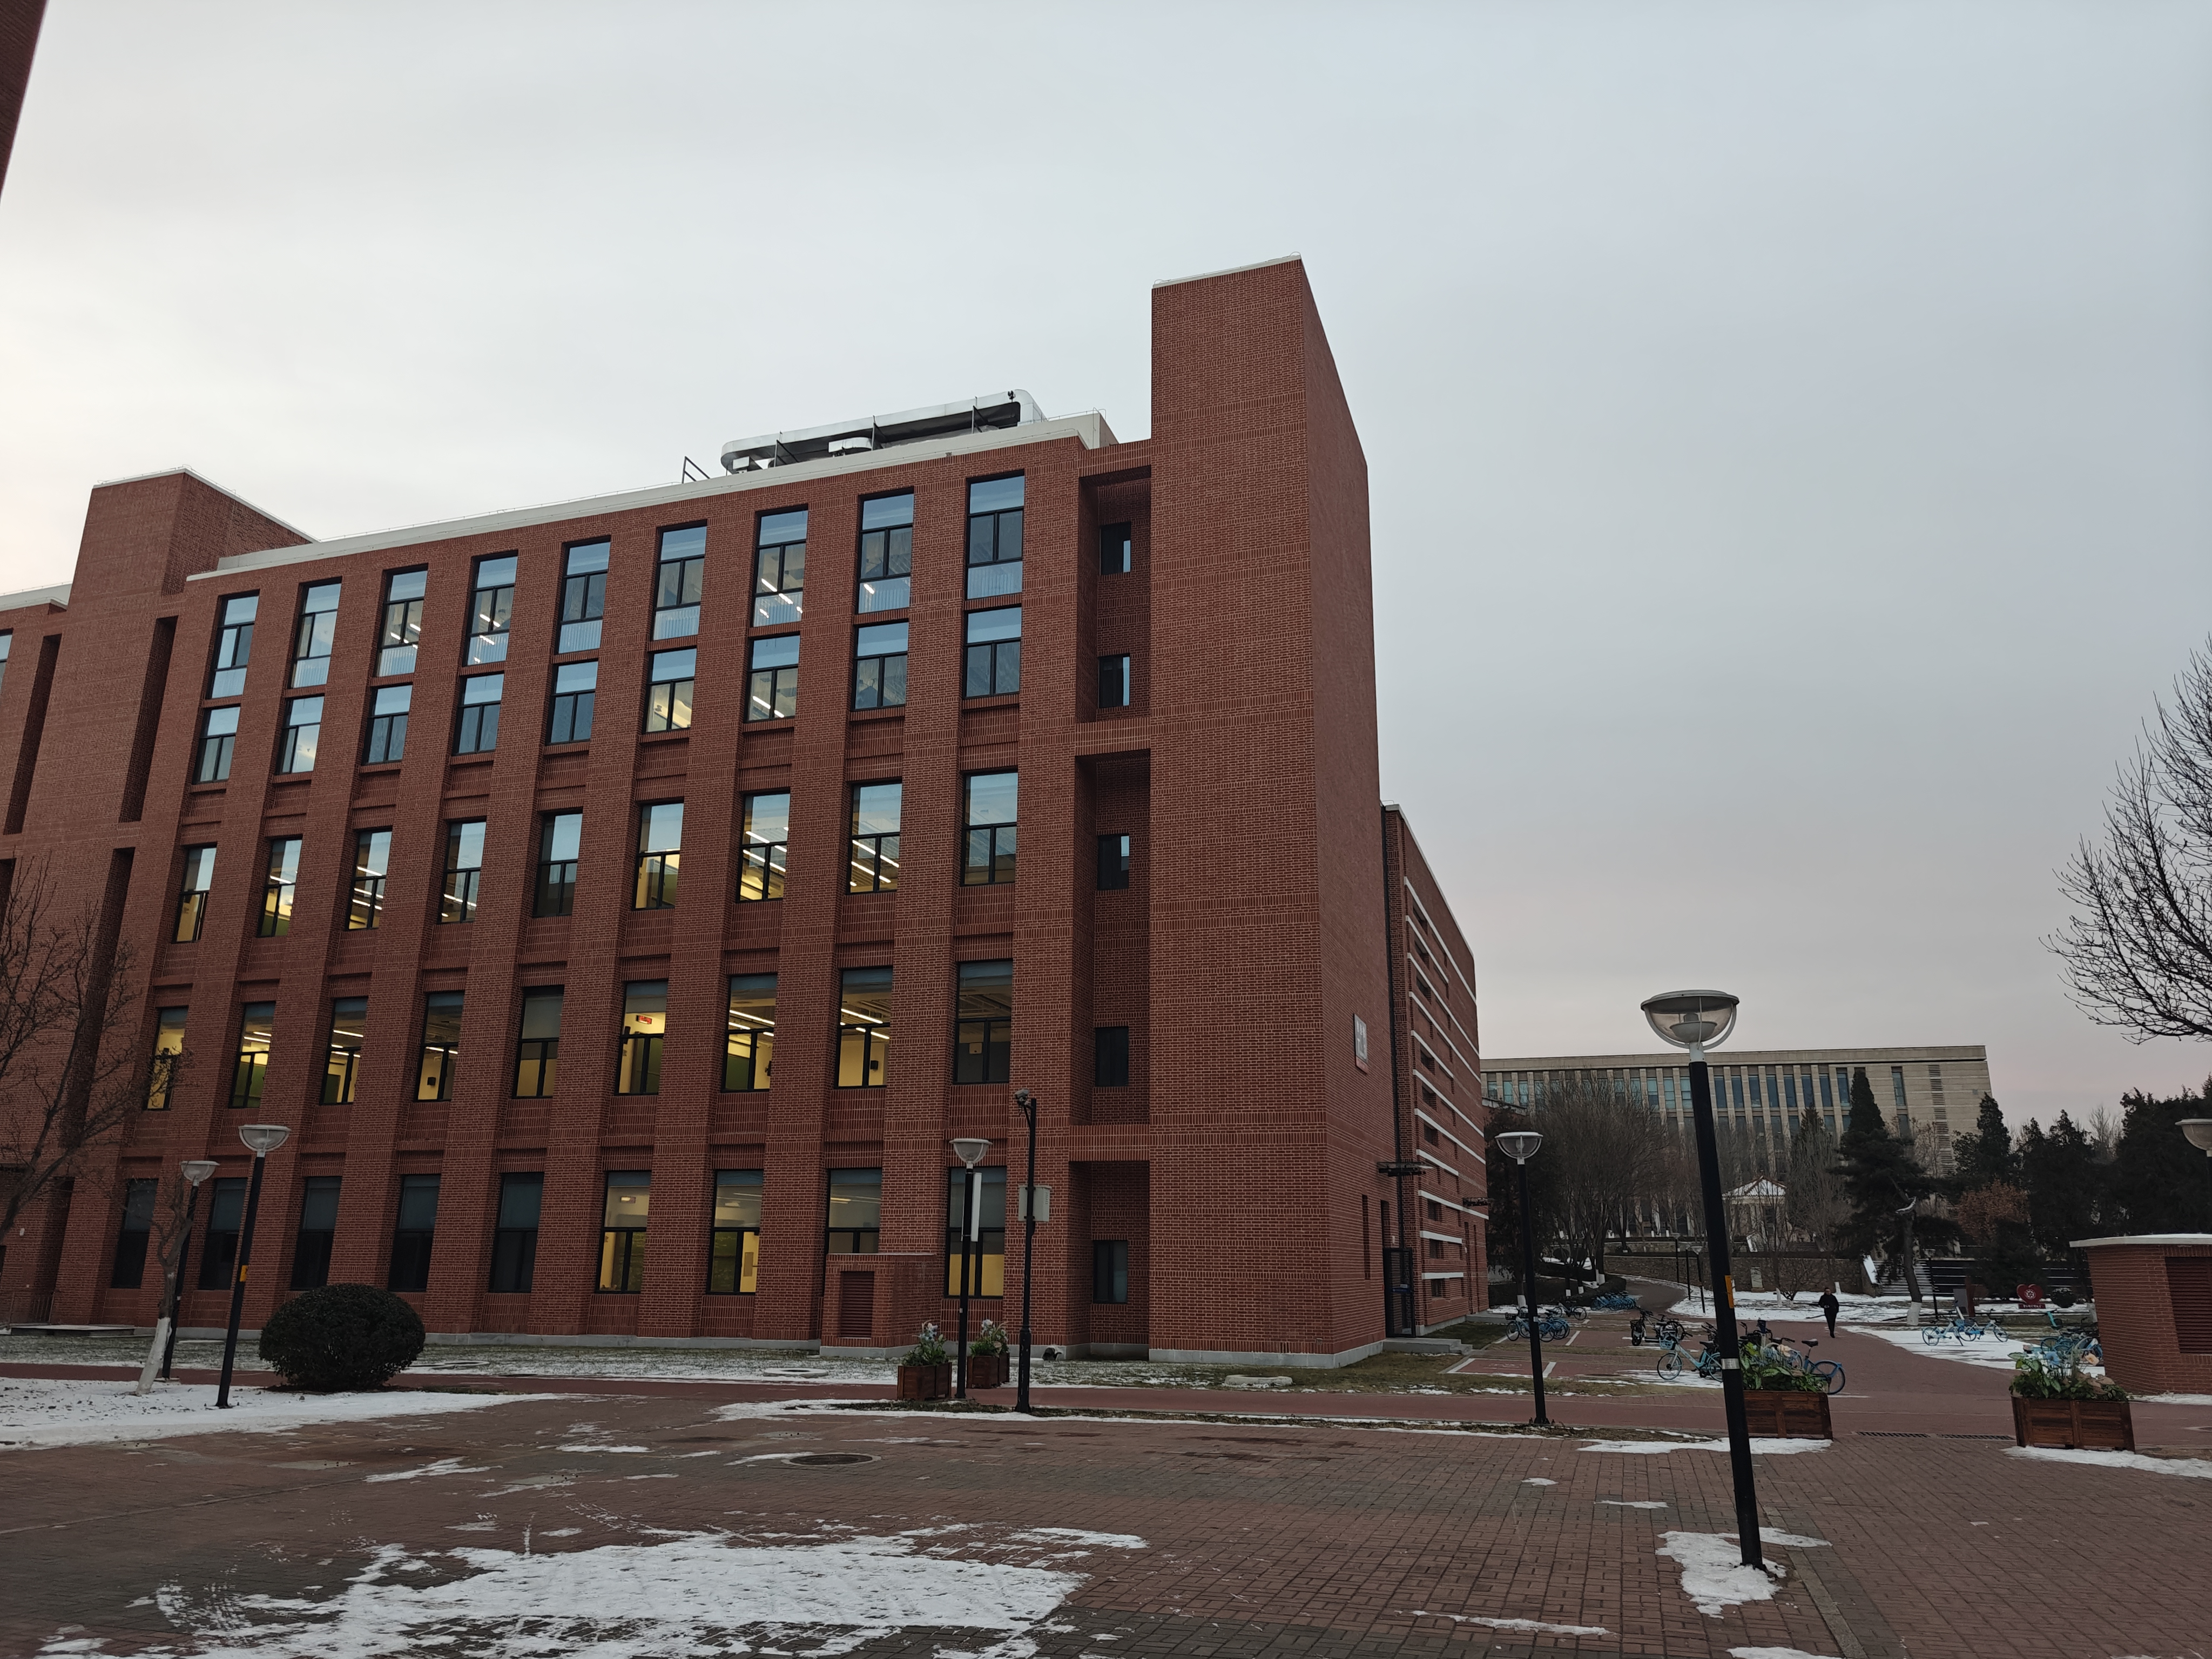
\includegraphics[width=\linewidth]{dataset/2.jpg}
        \caption{原图 (Original)}
    \end{subfigure}
    \hfill
    \begin{subfigure}{0.3\textwidth}
        \centering
        \includegraphics[width=\linewidth]{Ncutresults/ncut_2.jpg}
        \caption{Normalized Cuts}
    \end{subfigure}
    \hfill
    \begin{subfigure}{0.3\textwidth}
        \centering
        \includegraphics[width=\linewidth]{cityscapes_result/2_semantic.png}
        \caption{DeepLab (Cityscapes)}
    \end{subfigure}
    
    \vspace{1em}
    
    \begin{subfigure}{0.3\textwidth}
        \centering
        \includegraphics[width=\linewidth]{voc_results/2semantic.png}
        \caption{DeepLab (Pascal VOC)}
    \end{subfigure}
    \hfill
    \begin{subfigure}{0.3\textwidth}
        \centering
        \includegraphics[width=\linewidth]{SAMresults-vit_b/sam_2.png}
        \caption{SAM (ViT-B)}
    \end{subfigure}
    \hfill
    \begin{subfigure}{0.3\textwidth}
        \centering
        \includegraphics[width=\linewidth]{SAMresults-vit_h/sam2.png}
        \caption{SAM (ViT-H)}
    \end{subfigure}
    
    \caption{公开数据集测试用例 2}
    \label{fig:public_case2}
\end{figure}

% --- 测试用例 3 ---
\begin{figure}[htbp]
    \centering
    \begin{subfigure}{0.3\textwidth}
        \centering
        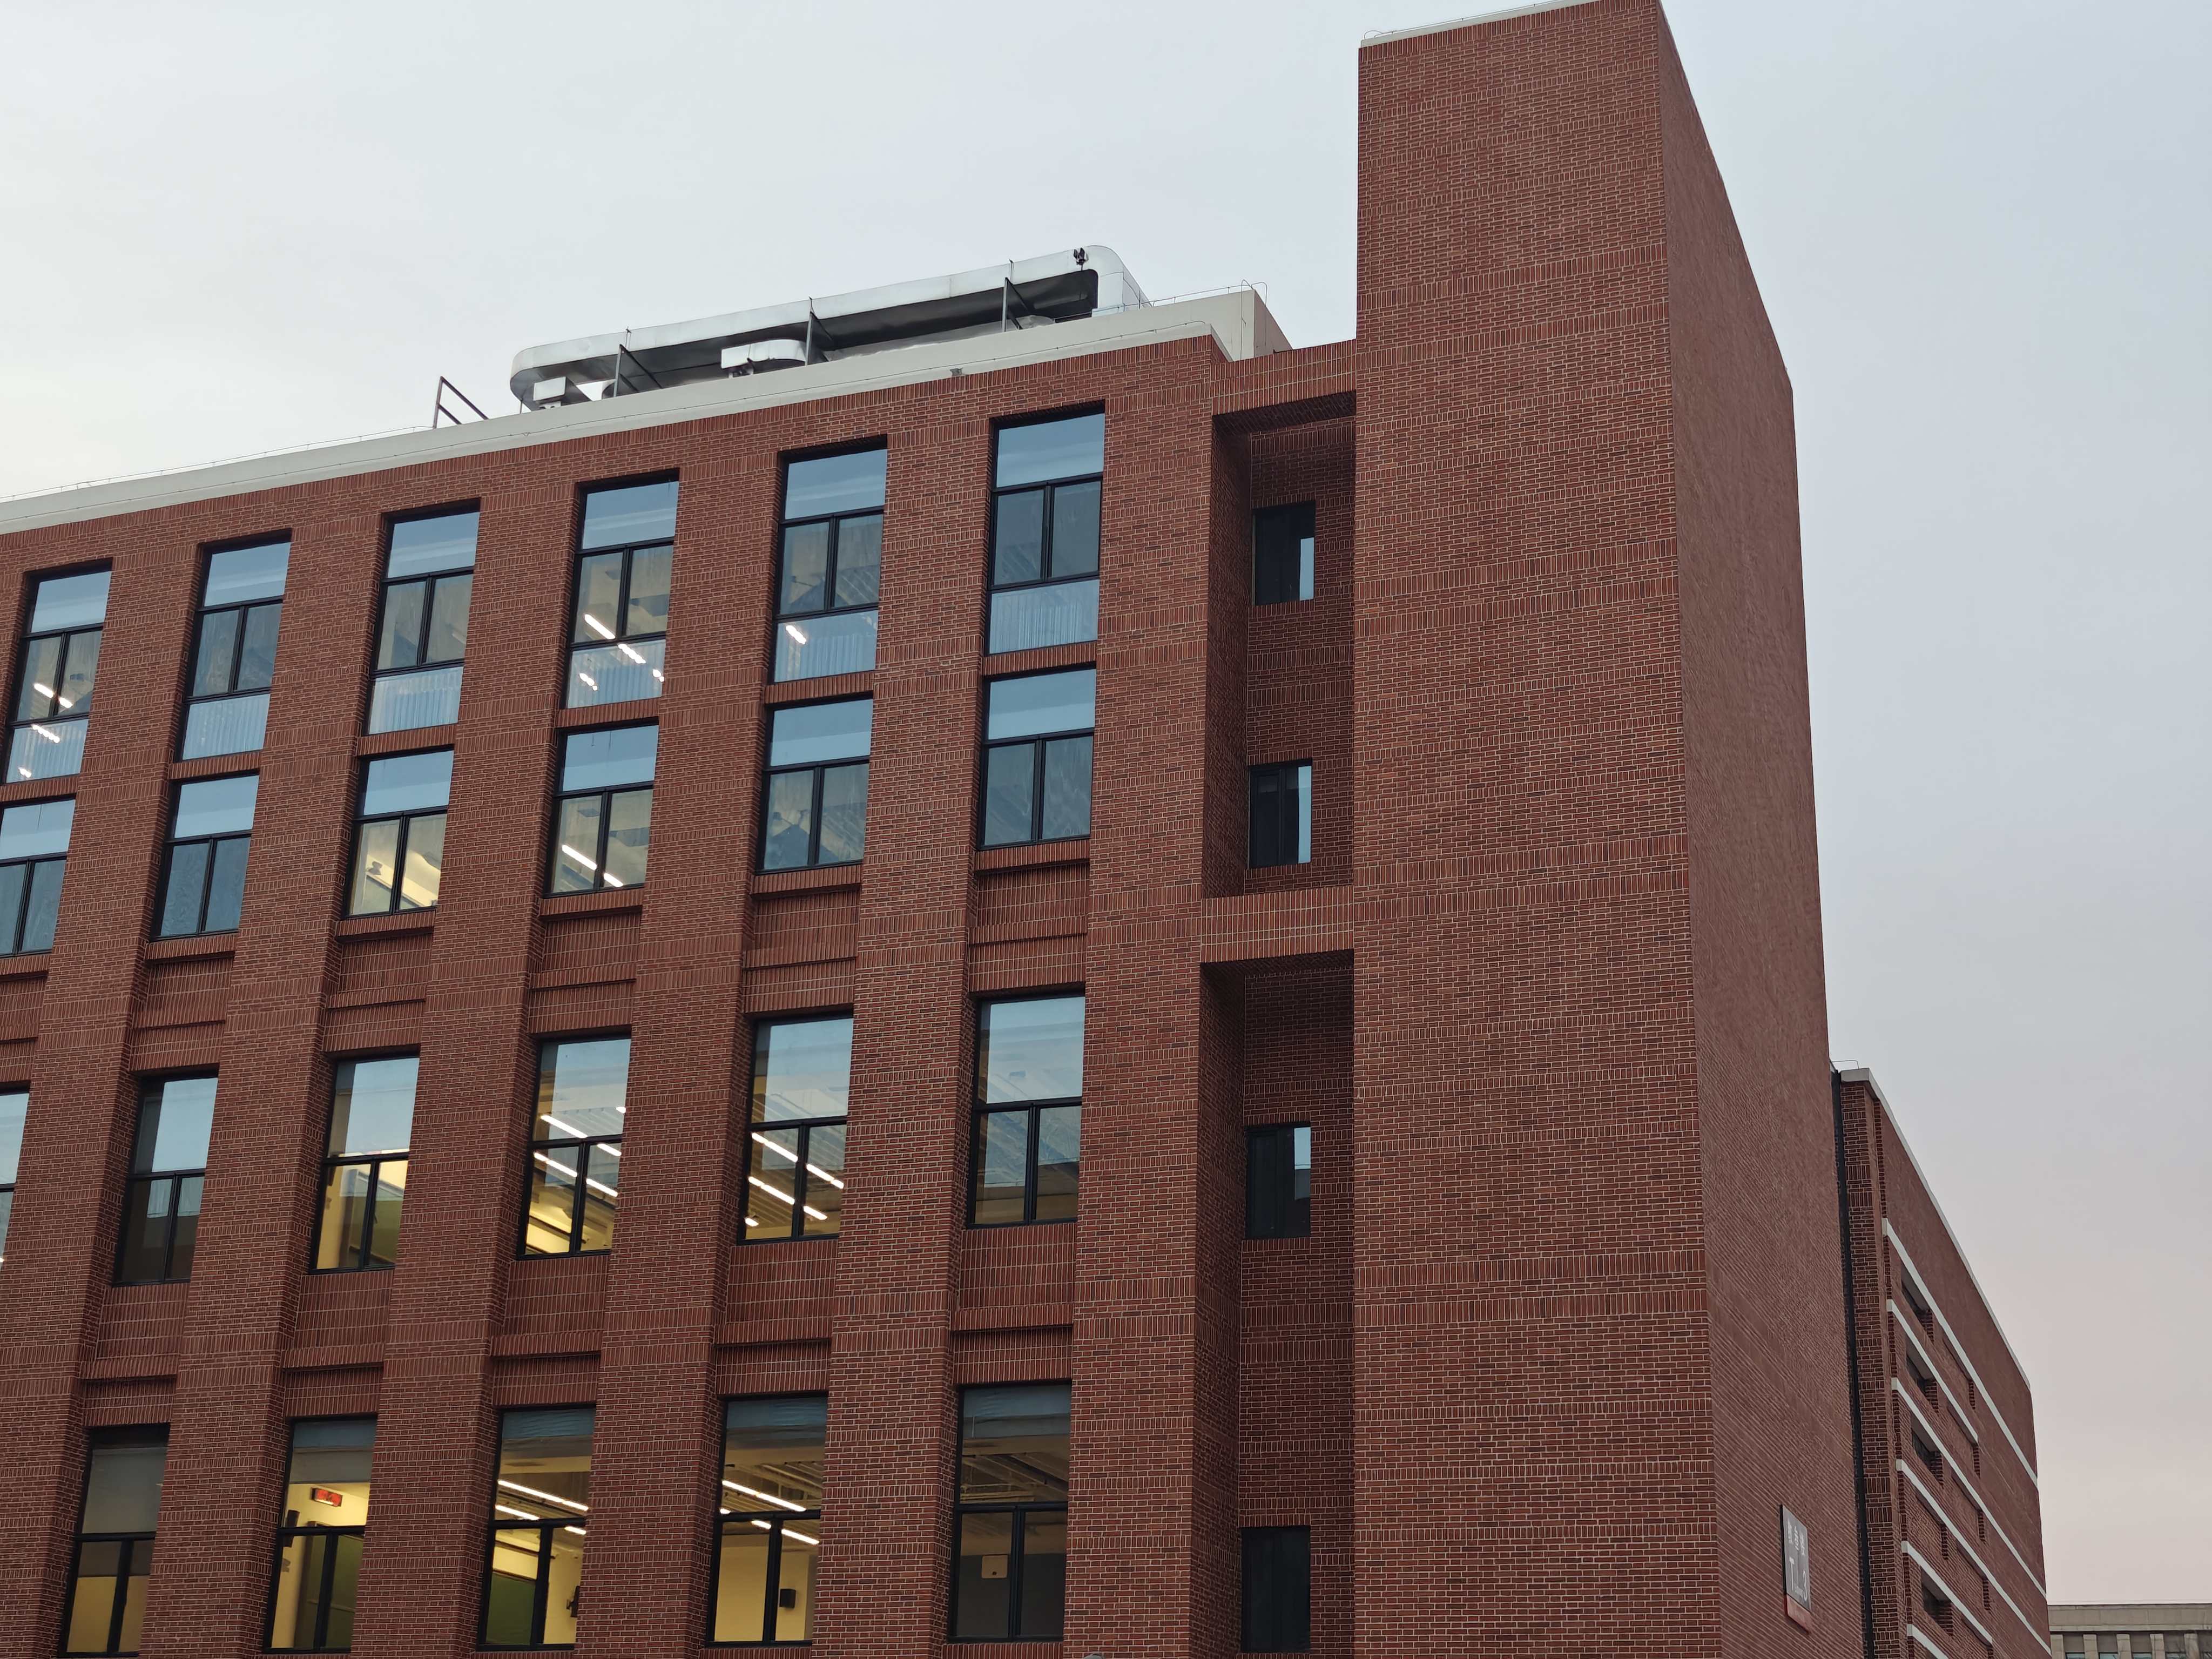
\includegraphics[width=\linewidth]{dataset/3.jpg}
        \caption{原图 (Original)}
    \end{subfigure}
    \hfill
    \begin{subfigure}{0.3\textwidth}
        \centering
        \includegraphics[width=\linewidth]{Ncutresults/ncut_3.jpg}
        \caption{Normalized Cuts}
    \end{subfigure}
    \hfill
    \begin{subfigure}{0.3\textwidth}
        \centering
        \includegraphics[width=\linewidth]{cityscapes_result/3_semantic.png}
        \caption{DeepLab (Cityscapes)}
    \end{subfigure}
    
    \vspace{1em}
    
    \begin{subfigure}{0.3\textwidth}
        \centering
        \includegraphics[width=\linewidth]{voc_results/3semantic.png}
        \caption{DeepLab (Pascal VOC)}
    \end{subfigure}
    \hfill
    \begin{subfigure}{0.3\textwidth}
        \centering
        \includegraphics[width=\linewidth]{SAMresults-vit_b/sam_3.png}
        \caption{SAM (ViT-B)}
    \end{subfigure}
    \hfill
    \begin{subfigure}{0.3\textwidth}
        \centering
        \includegraphics[width=\linewidth]{SAMresults-vit_h/sam3.png}
        \caption{SAM (ViT-H)}
    \end{subfigure}
    
    \caption{公开数据集测试用例 3}
    \label{fig:public_case3}
\end{figure}

% --- 测试用例 4 ---
\begin{figure}[htbp]
    \centering
    \begin{subfigure}{0.3\textwidth}
        \centering
        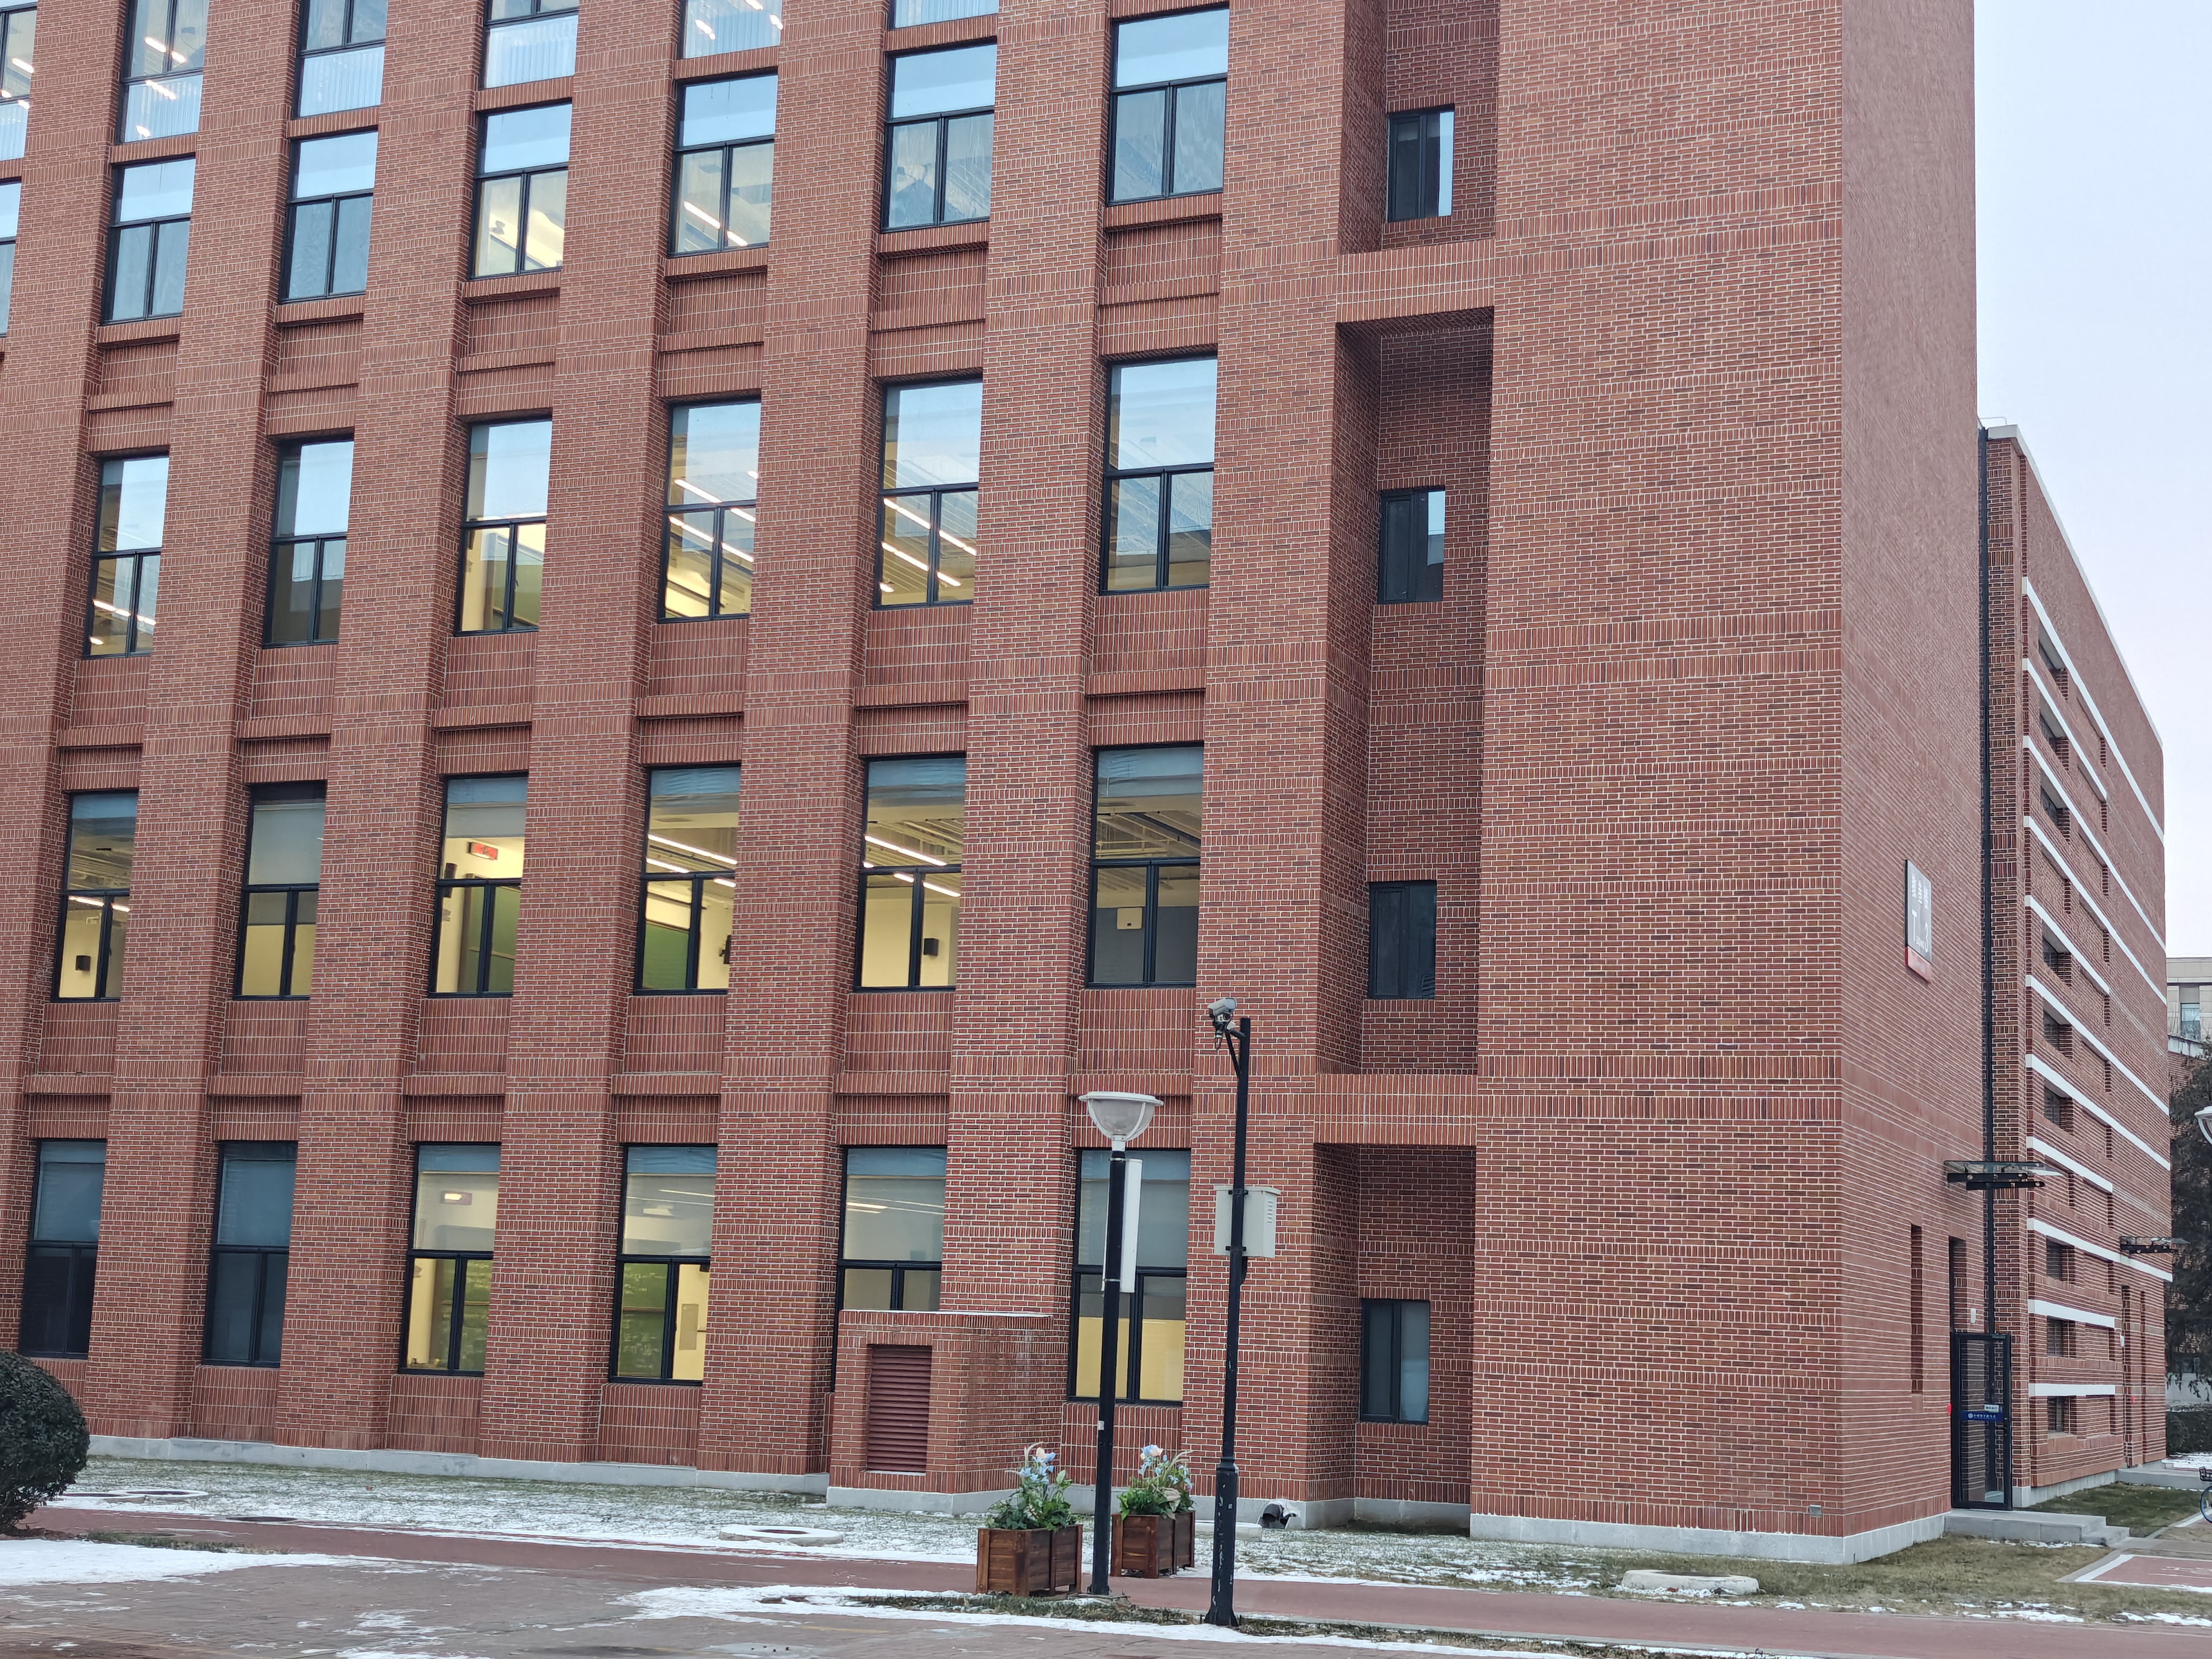
\includegraphics[width=\linewidth]{dataset/4.jpg}
        \caption{原图 (Original)}
    \end{subfigure}
    \hfill
    \begin{subfigure}{0.3\textwidth}
        \centering
        \includegraphics[width=\linewidth]{Ncutresults/ncut_4.jpg}
        \caption{Normalized Cuts}
    \end{subfigure}
    \hfill
    \begin{subfigure}{0.3\textwidth}
        \centering
        \includegraphics[width=\linewidth]{cityscapes_result/4_semantic.png}
        \caption{DeepLab (Cityscapes)}
    \end{subfigure}
    
    \vspace{1em}
    
    \begin{subfigure}{0.3\textwidth}
        \centering
        \includegraphics[width=\linewidth]{voc_results/4semantic.png}
        \caption{DeepLab (Pascal VOC)}
    \end{subfigure}
    \hfill
    \begin{subfigure}{0.3\textwidth}
        \centering
        \includegraphics[width=\linewidth]{SAMresults-vit_b/sam_4.png}
        \caption{SAM (ViT-B)}
    \end{subfigure}
    \hfill
    \begin{subfigure}{0.3\textwidth}
        \centering
        \includegraphics[width=\linewidth]{SAMresults-vit_h/sam4.png}
        \caption{SAM (ViT-H)}
    \end{subfigure}
    
    \caption{公开数据集测试用例 4}
    \label{fig:public_case4}
\end{figure}

\subsection{自采数据集测试结果}

% --- 测试用例 5 ---
\begin{figure}[H]
    \centering
    \begin{subfigure}{0.15\textwidth}
        \centering
        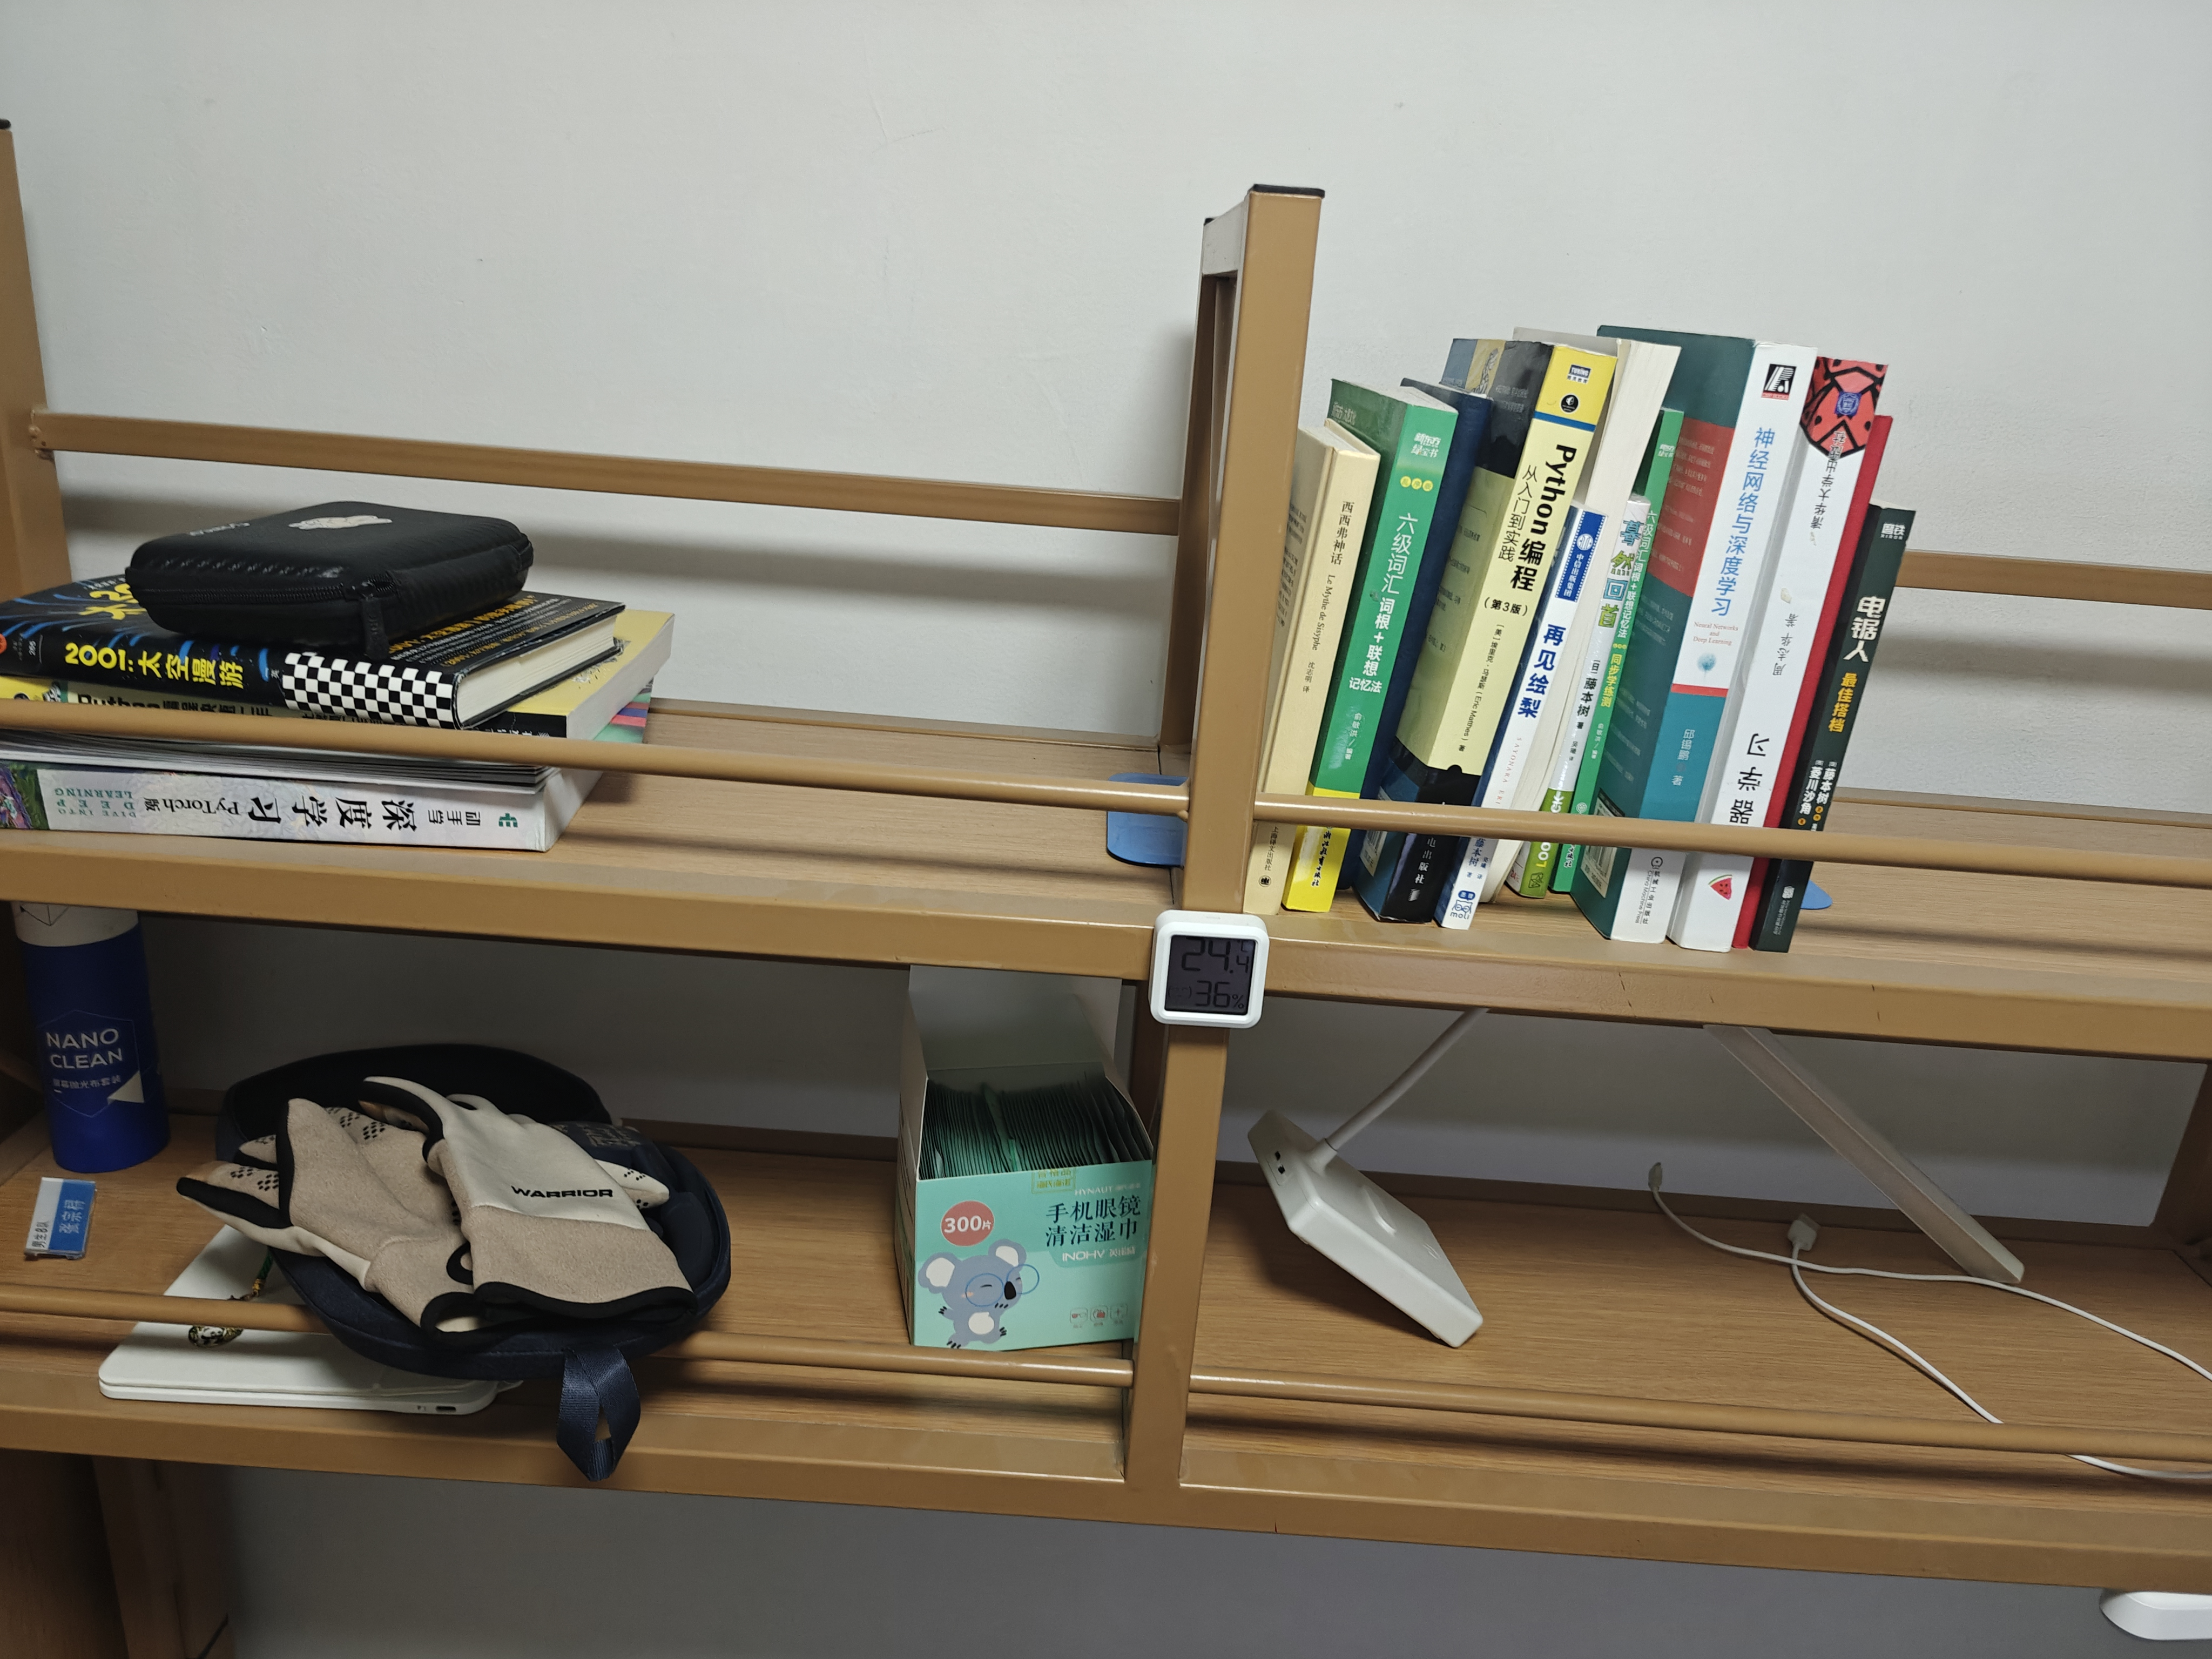
\includegraphics[width=\linewidth]{dataset/5.jpg}
        \caption{原图 (Original)}
    \end{subfigure}
    \hfill
    \begin{subfigure}{0.15\textwidth}
        \centering
        \includegraphics[width=\linewidth]{Ncutresults/ncut_5.jpg}
        \caption{Normalized Cuts}
    \end{subfigure}
    \hfill
    \begin{subfigure}{0.15\textwidth}
        \centering
        \includegraphics[width=\linewidth]{cityscapes_result/5_semantic.png}
        \caption{DeepLab (Cityscapes)}
    \end{subfigure}
    
    \vspace{1em}
    
    \begin{subfigure}{0.15\textwidth}
        \centering
        \includegraphics[width=\linewidth]{voc_results/5semantic.png}
        \caption{DeepLab (Pascal VOC)}
    \end{subfigure}
    \hfill
    \begin{subfigure}{0.15\textwidth}
        \centering
        \includegraphics[width=\linewidth]{SAMresults-vit_b/sam_5.png}
        \caption{SAM (ViT-B)}
    \end{subfigure}
    \hfill
    \begin{subfigure}{0.15\textwidth}
        \centering
        \includegraphics[width=\linewidth]{SAMresults-vit_h/sam5.png}
        \caption{SAM (ViT-H)}
    \end{subfigure}
    
    \caption{自采数据集测试用例 1}
    \label{fig:self_case1}
\end{figure}

% --- 测试用例 6 ---
\begin{figure}[htbp]
    \centering
    \begin{subfigure}{0.3\textwidth}
        \centering
        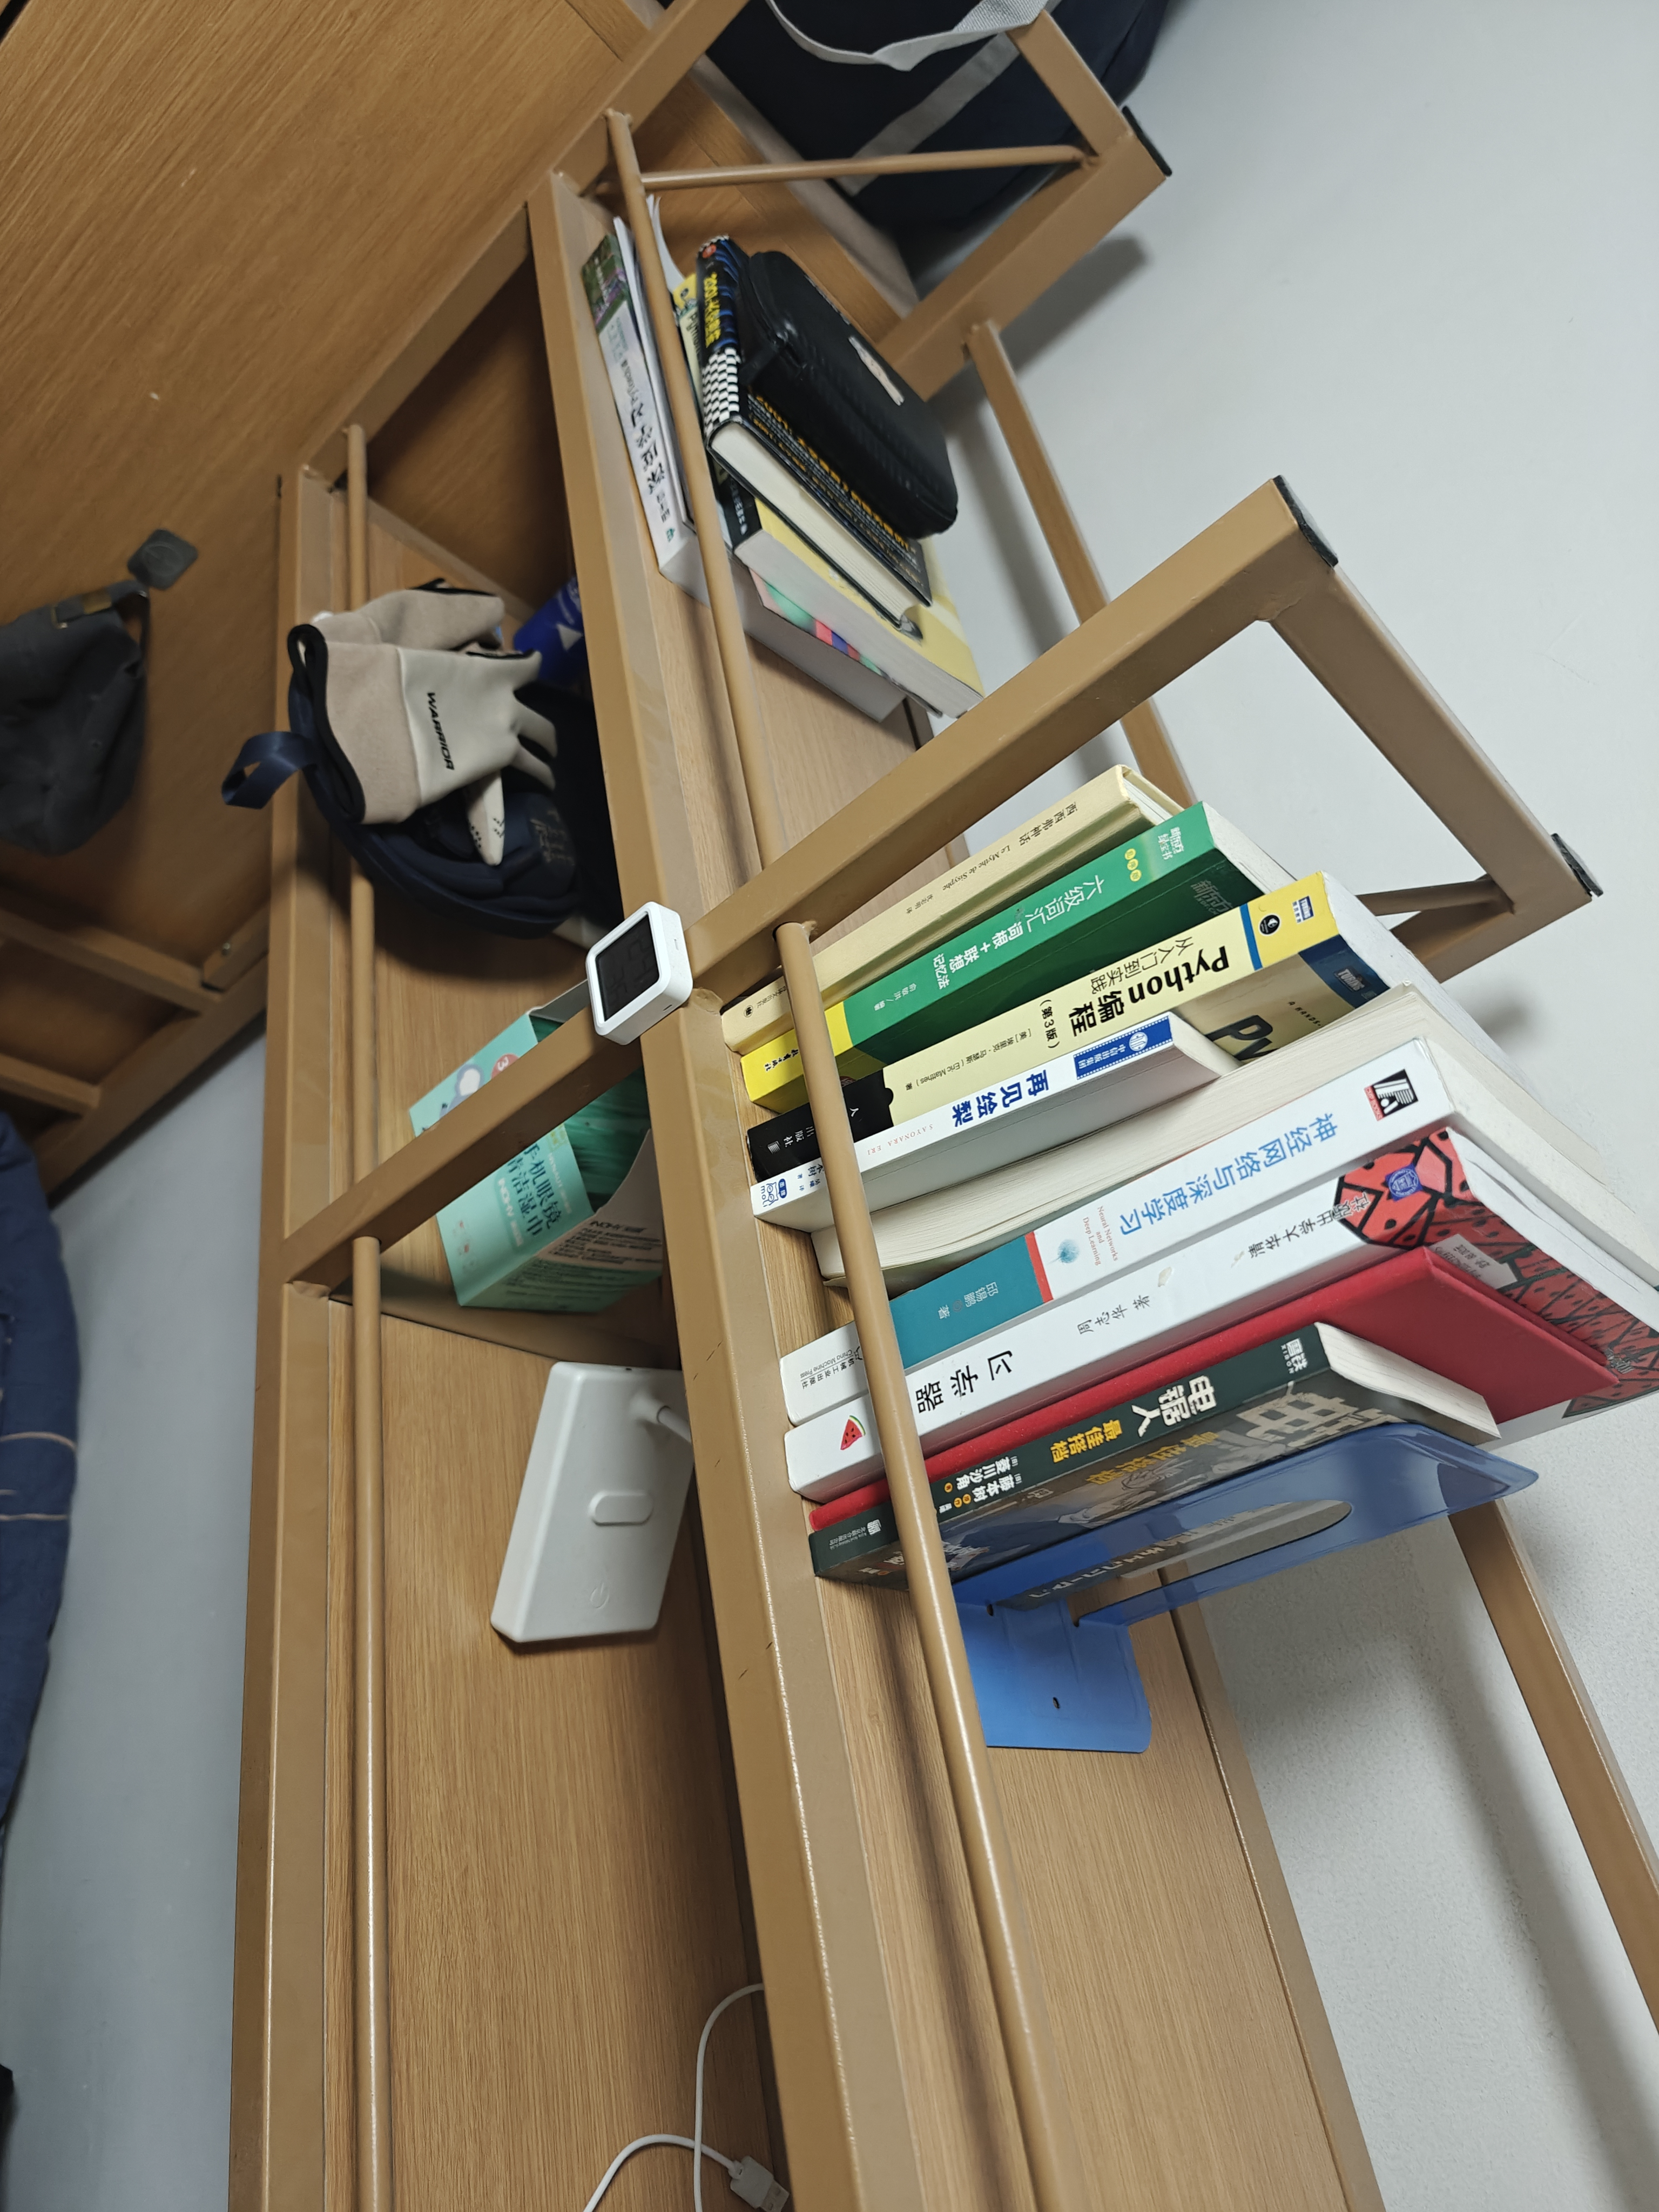
\includegraphics[width=\linewidth]{dataset/6.jpg}
        \caption{原图 (Original)}
    \end{subfigure}
    \hfill
    \begin{subfigure}{0.3\textwidth}
        \centering
        \includegraphics[width=\linewidth]{Ncutresults/ncut_6.jpg}
        \caption{Normalized Cuts}
    \end{subfigure}
    \hfill
    \begin{subfigure}{0.3\textwidth}
        \centering
        \includegraphics[width=\linewidth]{cityscapes_result/6_semantic.png}
        \caption{DeepLab (Cityscapes)}
    \end{subfigure}
    
    \vspace{1em}
    
    \begin{subfigure}{0.3\textwidth}
        \centering
        \includegraphics[width=\linewidth]{voc_results/6semantic.png}
        \caption{DeepLab (Pascal VOC)}
    \end{subfigure}
    \hfill
    \begin{subfigure}{0.3\textwidth}
        \centering
        \includegraphics[width=\linewidth]{SAMresults-vit_b/sam_6.png}
        \caption{SAM (ViT-B)}
    \end{subfigure}
    \hfill
    \begin{subfigure}{0.3\textwidth}
        \centering
        \includegraphics[width=\linewidth]{SAMresults-vit_h/sam6.png}
        \caption{SAM (ViT-H)}
    \end{subfigure}
    
    \caption{自采数据集测试用例 2}
    \label{fig:self_case2}
\end{figure}

% --- 测试用例 7 ---
\begin{figure}[htbp]
    \centering
    \begin{subfigure}{0.3\textwidth}
        \centering
        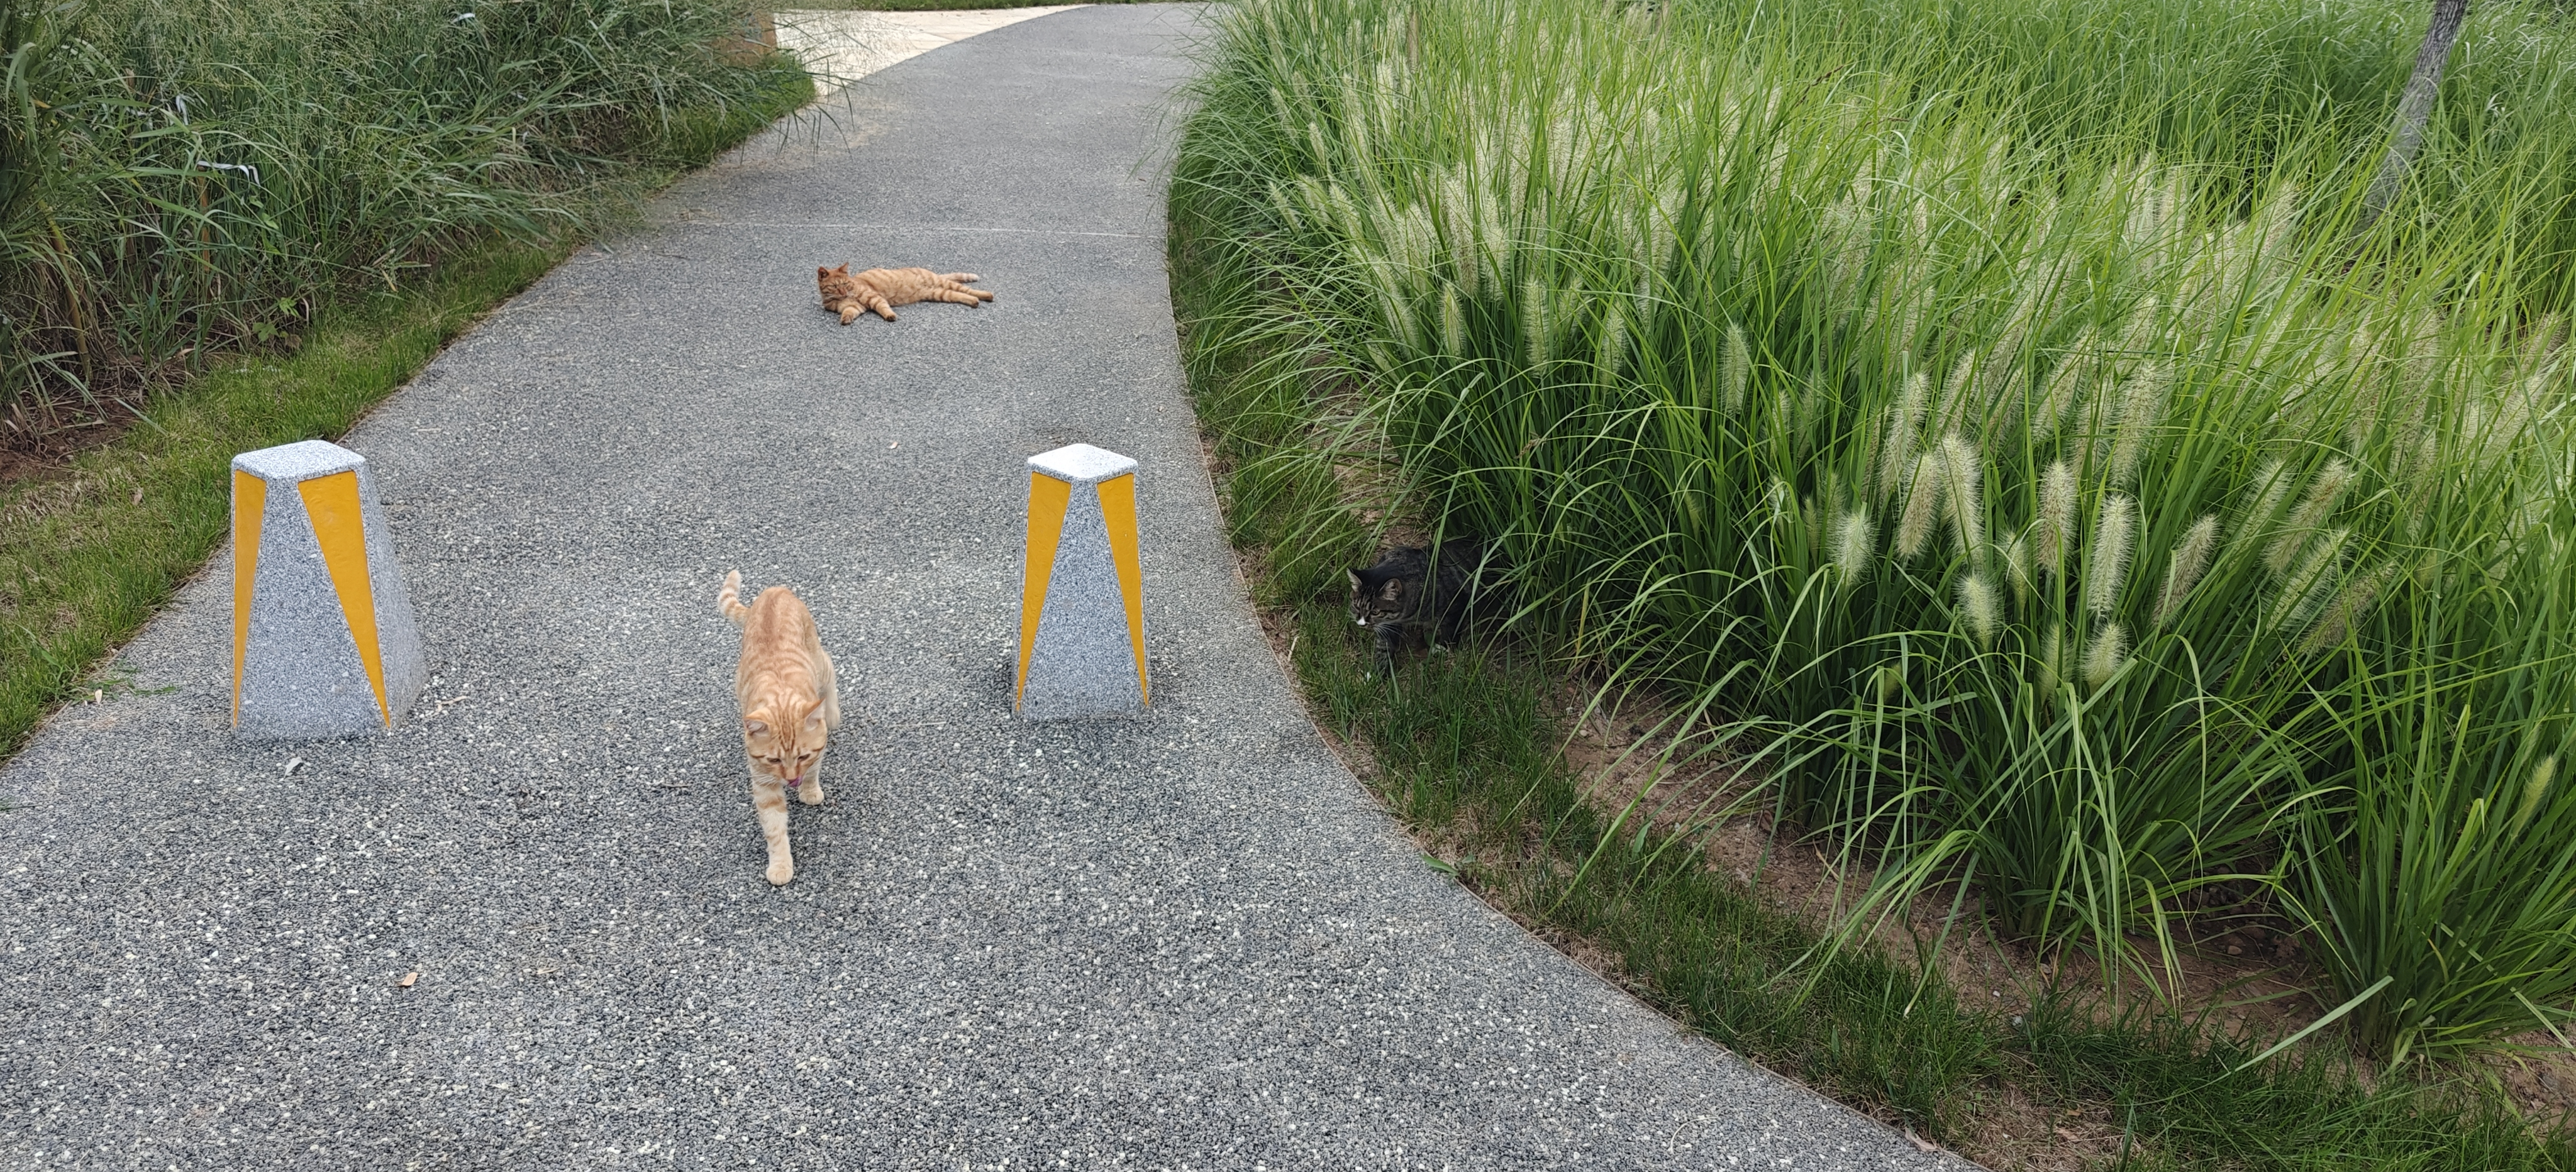
\includegraphics[width=\linewidth]{dataset/7.jpg}
        \caption{原图 (Original)}
    \end{subfigure}
    \hfill
    \begin{subfigure}{0.3\textwidth}
        \centering
        \includegraphics[width=\linewidth]{Ncutresults/ncut_7.jpg}
        \caption{Normalized Cuts}
    \end{subfigure}
    \hfill
    \begin{subfigure}{0.3\textwidth}
        \centering
        \includegraphics[width=\linewidth]{cityscapes_result/7_semantic.png}
        \caption{DeepLab (Cityscapes)}
    \end{subfigure}
    
    \vspace{1em}
    
    \begin{subfigure}{0.3\textwidth}
        \centering
        \includegraphics[width=\linewidth]{voc_results/7semantic.png}
        \caption{DeepLab (Pascal VOC)}
    \end{subfigure}
    \hfill
    \begin{subfigure}{0.3\textwidth}
        \centering
        \includegraphics[width=\linewidth]{SAMresults-vit_b/sam_7.png}
        \caption{SAM (ViT-B)}
    \end{subfigure}
    \hfill
    \begin{subfigure}{0.3\textwidth}
        \centering
        \includegraphics[width=\linewidth]{SAMresults-vit_h/sam7.png}
        \caption{SAM (ViT-H)}
    \end{subfigure}
    
    \caption{自采数据集测试用例 3}
    \label{fig:self_case3}
\end{figure}

% --- 测试用例 8 ---
\begin{figure}[H]
    \centering
    \begin{subfigure}{0.3\textwidth}
        \centering
        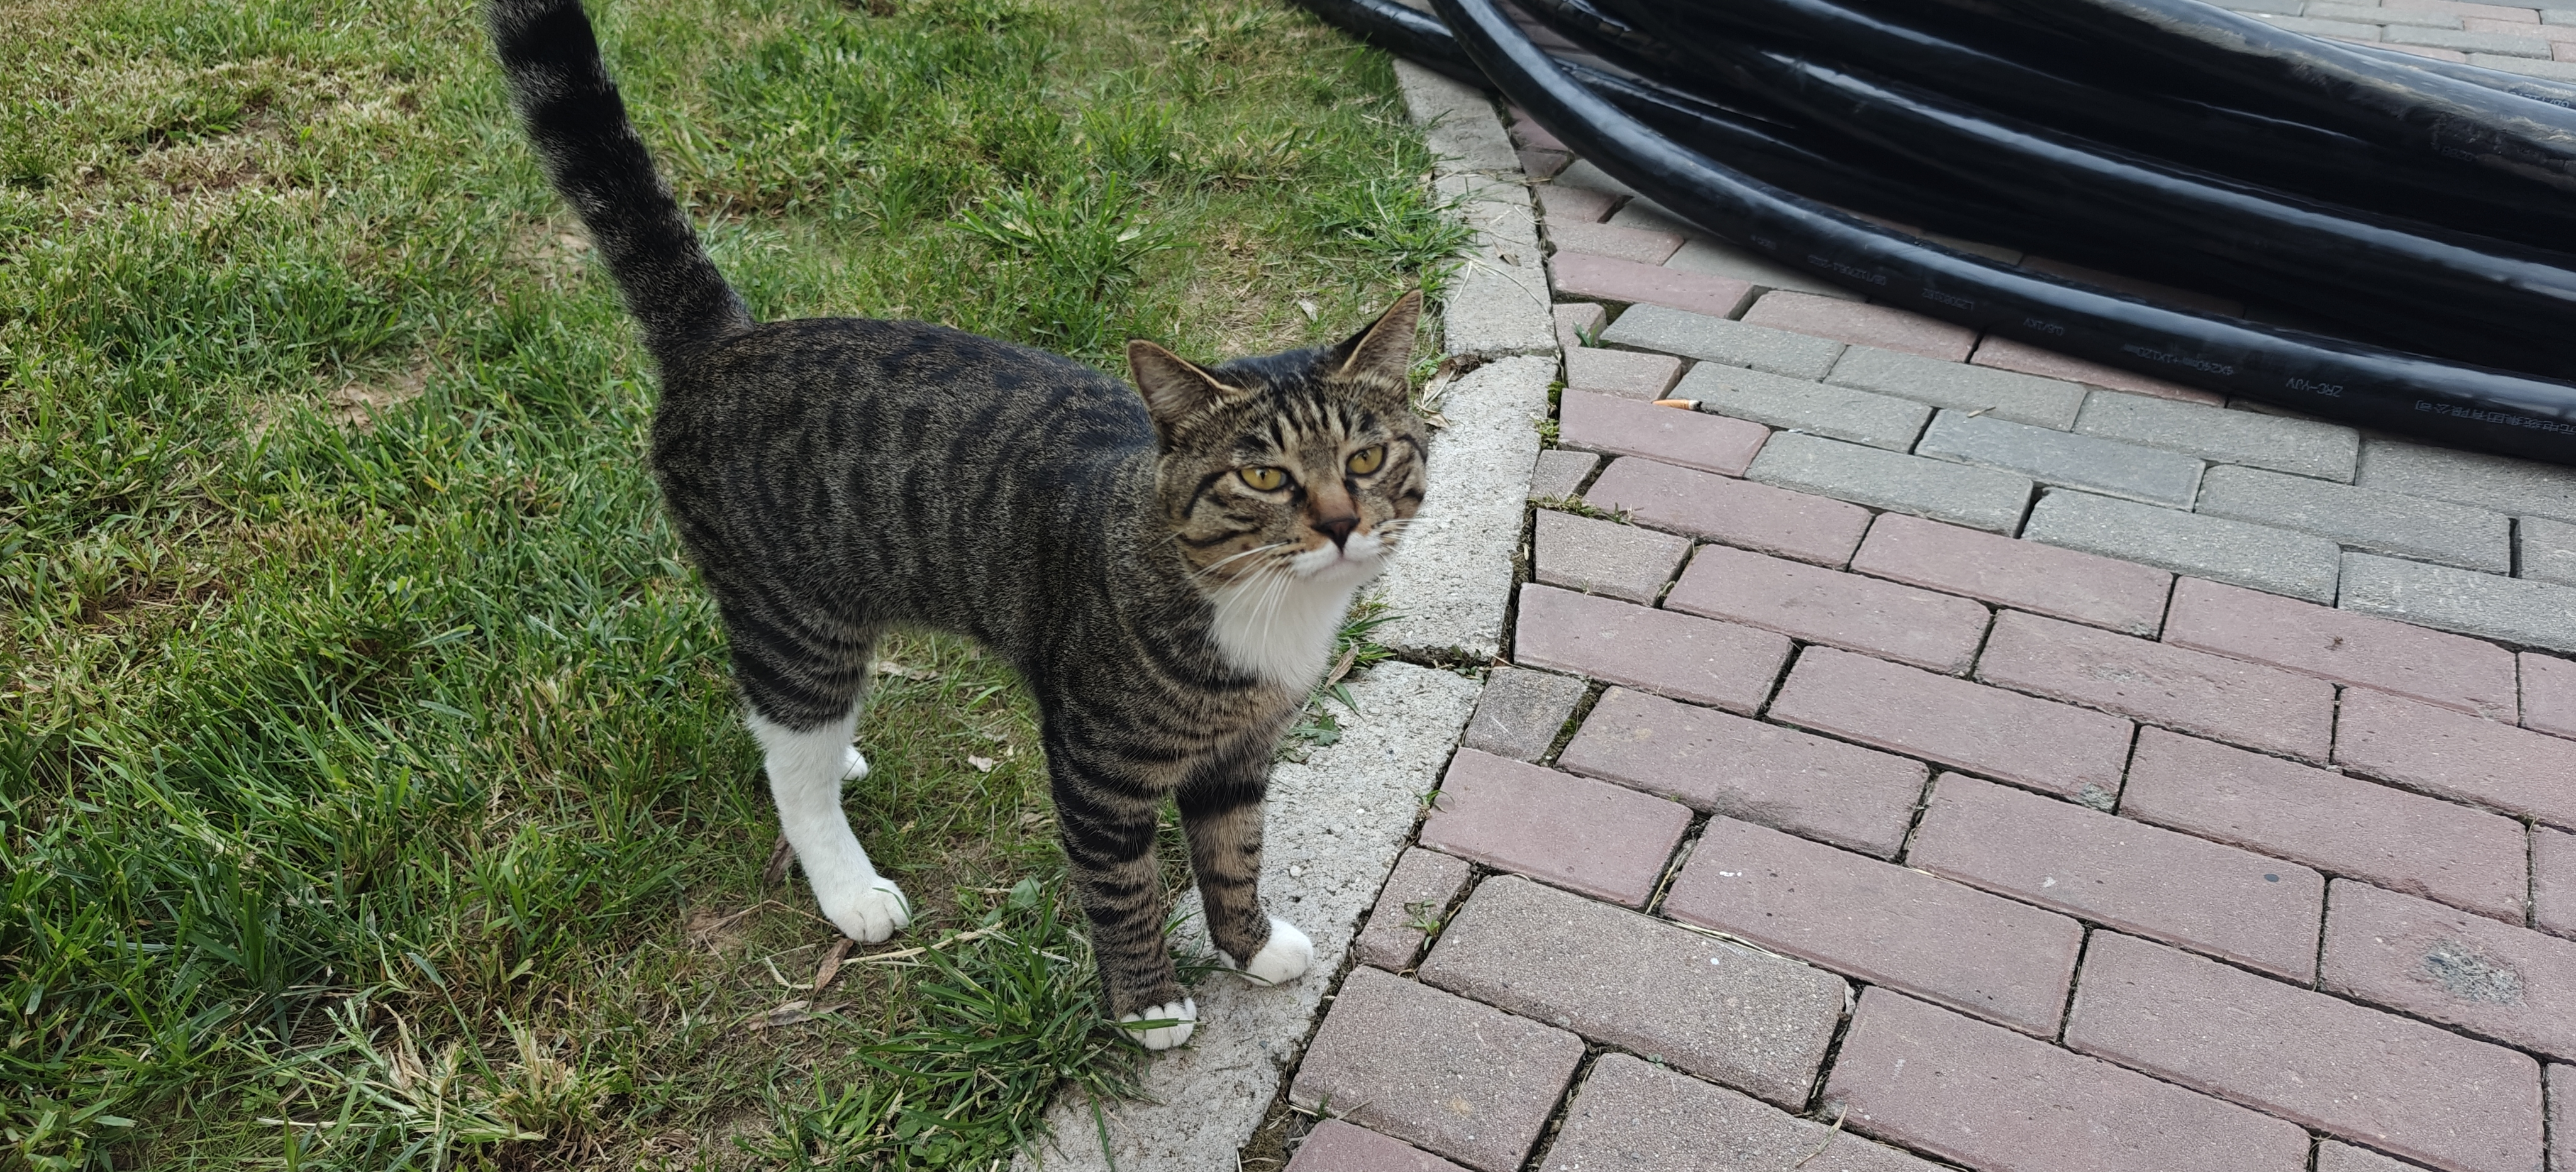
\includegraphics[width=\linewidth]{dataset/8.jpg}
        \caption{原图 (Original)}
    \end{subfigure}
    \hfill
    \begin{subfigure}{0.3\textwidth}
        \centering
        \includegraphics[width=\linewidth]{Ncutresults/ncut_8.jpg}
        \caption{Normalized Cuts}
    \end{subfigure}
    \hfill
    \begin{subfigure}{0.3\textwidth}
        \centering
        \includegraphics[width=\linewidth]{cityscapes_result/8_semantic.png}
        \caption{DeepLab (Cityscapes)}
    \end{subfigure}
    
    \vspace{1em}
    
    \begin{subfigure}{0.3\textwidth}
        \centering
        \includegraphics[width=\linewidth]{voc_results/8semantic.png}
        \caption{DeepLab (Pascal VOC)}
    \end{subfigure}
    \hfill
    \begin{subfigure}{0.3\textwidth}
        \centering
        \includegraphics[width=\linewidth]{SAMresults-vit_b/sam_8.png}
        \caption{SAM (ViT-B)}
    \end{subfigure}
    \hfill
    \begin{subfigure}{0.3\textwidth}
        \centering
        \includegraphics[width=\linewidth]{SAMresults-vit_h/sam8.png}
        \caption{SAM (ViT-H)}
    \end{subfigure}
    
    \caption{自采数据集测试用例 4}
    \label{fig:self_case4}
\end{figure}

\section{同类分析}
在这一部分,我们将对比DeepLab v3+ 与 SAM 在采用不同预训练模型时的表现。
\subsection{SAM模型}

SAM 是 Meta AI 提出的 Segment Anything Model (SAM) 作为图像分割的基础框架。SAM 旨在解决通用的图像分割任务,具有强大的零样本迁移能力,能够处理训练集中未见过的物体类别。

SAM 的网络架构由三个主要部分组成,设计上实现了高效的推理:
\begin{itemize}
    \item \textbf{图像编码器:} 基于 Vision Transformer (ViT) 架构,负责将输入图像映射为特征嵌入。这是模型中计算量最大的部分,但对每张图像仅需计算一次。
    \item \textbf{提示编码器:} 这是一个轻量级模块,用于将用户的交互提示(如点、框、掩码或文本)转换为提示向量。
    \item \textbf{掩码解码器:} 该模块将图像特征与提示特征相结合,通过轻量级的计算实时生成最终的分割掩码。
\end{itemize}

\subsubsection{权重文件对比:ViT-B 与 ViT-H}
SAM 的不同模型版本主要区别在于图像编码器的大小。本研究使用了官方提供的两个具有代表性的权重文件进行对比实验:\textbf{ViT-B (Base)} 和 \textbf{ViT-H (Huge)}。

\begin{itemize}
    \item \textbf{ViT-B (Base):} 这是一个基础版本的模型权重。它的参数量相对较小,推理速度快,内存占用低。在资源受限或对实时性要求较高的场景中,ViT-B 通常是首选。
    \item \textbf{ViT-H (Huge):} 这是 SAM 系列中规模最大、性能最强的版本。它拥有巨大的参数量,能够提取更丰富的图像特征。虽然其计算成本显著增加,但在处理复杂场景、模糊边界以及细小物体时,ViT-H 通常能提供更精细的分割质量。
\end{itemize}
\subsubsection{实验结果与分析}

为了评估模型容量对分割性能的具体影响,我们在室内复杂背景、多人物实例以及自然景观三种典型场景下,对比了 ViT-B (Base) 与 ViT-H (Huge) 两个不同量级权重的表现。实验采取仅显示最大的5个掩码作为输出。

\subsubsubsection{前景主体与背景识别}


\begin{figure}[H]
    \centering
    % 左列:ViT-B 结果
    \begin{subfigure}[b]{0.48\textwidth}
        \centering
        % TODO: 请在此处替换为【sam_3】的图片路径
        \includegraphics[width=\textwidth]{SAMresults-vit_b/sam_3.png}
        \caption{ViT-B 分割结果}
        \label{fig:cat_vitb}
    \end{subfigure}
    \hfill
    % 右列:ViT-H 结果
    \begin{subfigure}[b]{0.48\textwidth}
        \centering
        % TODO: 请在此处替换为【sam3】的图片路径
        \includegraphics[width=\textwidth]{SAMresults-vit_h/sam3.png}
        \caption{ViT-H 分割结果}
        \label{fig:cat_vith}
    \end{subfigure}
    \caption{室内复杂光影背景对比}
    \label{fig:cat_comparison}
\end{figure}

如图~\ref{fig:cat_comparison} 所示,两者表现差异巨大。\textbf{ViT-B} (图a) 显然受到了背景中高对比度图案的干扰,其“Top 5”分割结果主要集中在画面两侧的彩色条纹(紫色、绿色、红色块),而作为画面的真正主体——猫,却几乎融入背景。相比之下,\textbf{ViT-H} (图b) 展现了较好的语义聚焦能力,它成功抑制了背景噪声的干扰,将画面中央的猫识别为最显著的单一对象(亮紫色区域),且轮廓完整清晰。

\subsubsubsection{人物实例}

\begin{figure}[H]
    \centering
    % 左列:ViT-B 结果
    \begin{subfigure}[b]{0.48\textwidth}
        \centering
        % TODO: 请在此处替换为【sam_5】的图片路径
        \includegraphics[width=\textwidth]{SAMresults-vit_b/sam_5.png}
        \caption{ViT-B 分割结果}
        \label{fig:people_vitb}
    \end{subfigure}
    \hfill
    % 右列:ViT-H 结果
    \begin{subfigure}[b]{0.48\textwidth}
        \centering
        % TODO: 请在此处替换为【sam5】的图片路径
        \includegraphics[width=\textwidth]{SAMresults-vit_h/sam5.png}
        \caption{ViT-H 分割结果}
        \label{fig:people_vith}
    \end{subfigure}
    \caption{草地背景下多人目标对比}
    \label{fig:people_comparison}
\end{figure}

对比图~\ref{fig:people_comparison} 可以看出,\textbf{ViT-B} 在语义理解上存在碎片化问题。它未能理解肢体与躯干的从属关系,错误地将左侧球员举起的手臂丢失,并将右侧球员分割为上下两部分。而 \textbf{ViT-H} 表现出极强的语义连通性,准确地将头部、躯干和四肢识别为同一个实例,证明了其具备更深层的语义理解能力。

\subsubsubsection{自然景观}

\begin{figure}[H]
    \centering
    % 左列:ViT-B 结果
    \begin{subfigure}[b]{0.48\textwidth}
        \centering
        % TODO: 请在此处替换为【sam_7】的图片路径
        \includegraphics[width=\textwidth]{SAMresults-vit_b/sam_7.png}
        \caption{ViT-B 分割结果}
        \label{fig:park_vitb}
    \end{subfigure}
    \hfill
    % 右列:ViT-H 结果
    \begin{subfigure}[b]{0.48\textwidth}
        \centering
        % TODO: 请在此处替换为【sam6】的图片路径
        \includegraphics[width=\textwidth]{SAMresults-vit_h/sam6.png}
        \caption{ViT-H 分割结果}
        \label{fig:park_vith}
    \end{subfigure}
    \caption{户外路径下多小目标对比}
    \label{fig:park_comparison}
\end{figure}

如图~\ref{fig:park_comparison} 所示,\textbf{ViT-B} 生成的掩码显得杂乱且缺乏明确语义,仅覆盖了草坪的局部碎片。相反,\textbf{ViT-H} 能够结合全局上下文信息,生成了覆盖整块左侧草坪的完整掩码,且掩码边缘沿着硬质路面切分得非常整齐。这说明 ViT-H 在处理低纹理区域时具有更好的鲁棒性和区域一致性。

\subsubsection{结论}
综合上述实验,从 ViT-B 升级至 ViT-H 带来了显著的性能提升。具体表现在:
\begin{enumerate}
    \item \textbf{抗干扰能力:} ViT-H 能有效区分前景主体与背景高频噪声(如实验一中的猫与背景条纹)。
    \item \textbf{语义完整性:} ViT-H 能更好地理解物体的结构,避免将同一物体分割破碎(如实验二中的人物)。
    \item \textbf{区域一致性:} 在低纹理区域,ViT-H 能生成更符合人类认知的完整掩码(如实验三中的草地)。
\end{enumerate}

\subsection{DeepLabV3+ 模型}
DeepLabV3+ 是由 Google 团队提出的经典语义分割网络,其核心架构包含两个关键特性:
\begin{itemize}
    \item \textbf{空洞空间金字塔池化 :} 通过不同采样率的空洞卷积捕捉多尺度的上下文信息,显著提升了模型对不同大小物体的识别能力。
    \item \textbf{编解码器结构 :} 引入了简单的解码器模块。编码器提取丰富的高层语义特征,而解码器通过上采样并将低层细节特征与高层语义特征融合,有效地恢复了物体的空间分辨率和边界细节。
\end{itemize}

这种设计使得 DeepLabV3+ 在保持较高分割精度的同时,能够生成边缘更加锐利的分割结果。

\subsubsection{权重文件对比:Pascal VOC 与 Cityscapes}
本实验对比了分别在 Pascal VOC 和 Cityscapes 数据集上训练的两个权重文件,它们决定了模型能够识别的语义类别。

\begin{itemize}
    \item \textbf{Pascal VOC 权重:} 该权重在 PASCAL VOC 2012 数据集上训练。它侧重于\textbf{通用物体分割},包含 20 个前景类别(如人、猫、狗、椅子、飞机、汽车等)和 1 个背景类。该模型适合处理生活中常见的独立物体,注重物体层面的实例区分。
    \item \textbf{Cityscapes 权重:} 该权重在 Cityscapes 数据集上训练。它专注于\textbf{城市自动驾驶场景},包含 19 个语义类别(如道路、人行道、建筑、墙、交通标志、车辆、行人等)。该模型不仅关注前景物体,还关注背景环境(如天空、地面)的语义解析,适合处理复杂的街景图像。
\end{itemize}

\subsubsection{实验结果与分析}

不同于 SAM 模型中模型容量带来的差异,DeepLabV3+ 的对比实验主要揭示了预训练数据集(Pascal VOC 与 Cityscapes)对模型语义认知范围的影响。

\subsubsubsection{城市街景场景解析}

\begin{figure}[H]
    \centering
    % 左列:Pascal VOC 结果 (不带下划线)
    \begin{subfigure}[b]{0.48\textwidth}
        \centering
        % TODO: 请替换为 4semantic.png
        \includegraphics[width=\textwidth]{voc_results/4semantic.png}
        \caption{Pascal VOC 权重结果}
        \label{fig:street_voc}
    \end{subfigure}
    \hfill
    % 右列:Cityscapes 结果 (带下划线)
    \begin{subfigure}[b]{0.48\textwidth}
        \centering
        % TODO: 请替换为 4_semantic.png
        \includegraphics[width=\textwidth]{cityscapes_result/4_semantic.png}
        \caption{Cityscapes 权重结果}
        \label{fig:street_city}
    \end{subfigure}
    \caption{城市道路驾驶场景对比}
    \label{fig:deeplab_street}
\end{figure}

如图~\ref{fig:deeplab_street} 所示,两者差异显著。\textbf{Pascal VOC 权重} (图a) 表现为稀疏的物体检测,仅将画面中的车辆识别为前景(灰色区域),而将道路、树木和天空均视为背景(黑色)。这是因为 VOC 数据集主要针对特定物体类别的实例分割。相反,\textbf{Cityscapes 权重} (图b) 展现了密集的语义分割能力,正确将像素分类为道路(紫色)、植被(绿色)、天空(蓝色)和车辆(深蓝色),提供了完整的环境语义信息。

\subsubsubsection{室内物体泛化能力}

\begin{figure}[H]
    \centering
    % 左列:Pascal VOC 结果
    \begin{subfigure}[b]{0.48\textwidth}
        \centering
        % TODO: 请替换为 1semantic.png
        \includegraphics[width=\textwidth]{voc_results/1semantic.png}
        \caption{Pascal VOC 权重结果}
        \label{fig:flower_voc}
    \end{subfigure}
    \hfill
    % 右列:Cityscapes 结果
    \begin{subfigure}[b]{0.48\textwidth}
        \centering
        % TODO: 请替换为 1_semantic.png
        \includegraphics[width=\textwidth]{cityscapes_result/1_semantic.png}
        \caption{Cityscapes 权重结果}
        \label{fig:flower_city}
    \end{subfigure}
    \caption{复杂静物(瓶中花)对比}
    \label{fig:deeplab_flower}
\end{figure}

图~\ref{fig:deeplab_flower} 展示了严重的领域偏移现象。\textbf{Pascal VOC 权重} (图a) 准确地将花卉识别为“盆栽/植物”类别(绿色掩码),覆盖完整。然而,\textbf{Cityscapes 权重} (图b) 产生了严重的“幻觉”,将花卉错误地强制分类为各种杂乱的街景类别碎片。

\subsubsubsection{自然景观}

\begin{figure}[H]
    \centering
    % 左列:Pascal VOC 结果
    \begin{subfigure}[b]{0.48\textwidth}
        \centering
        % TODO: 请替换为 6semantic.png
        \includegraphics[width=\textwidth]{voc_results/6semantic.png}
        \caption{Pascal VOC 权重结果}
        \label{fig:park_voc}
    \end{subfigure}
    \hfill
    % 右列:Cityscapes 结果
    \begin{subfigure}[b]{0.48\textwidth}
        \centering
        % TODO: 请替换为 6_semantic.png
        \includegraphics[width=\textwidth]{cityscapes_result/6_semantic.png}
        \caption{Cityscapes 权重结果}
        \label{fig:park_city}
    \end{subfigure}
    \caption{户外景观对比}
    \label{fig:deeplab_park}
\end{figure}

在图~\ref{fig:deeplab_park} 中,\textbf{Pascal VOC 权重} (图a) 几乎输出全黑结果,主要是因为它不包含“草地”、“路面”或“天空”等背景类别,只能忽略。而 \textbf{Cityscapes 权重} (图b) 凭借对室外场景的先验知识,清晰地分割出了草地(亮绿色)、远山与树木(深绿色),以及天空(蓝色)。

\subsubsection{结论}
对于 DeepLabV3+ 而言,权重的选择应严格取决于应用场景:
\begin{enumerate}
    \item 若任务涉及\textbf{通用物体检测}(如机器人抓取、相册分类),应选择涵盖 20 类常见物体的 \textbf{Pascal VOC} 权重。
    \item 若任务涉及\textbf{自动驾驶或环境感知},需要理解道路布局和背景,则必须使用 \textbf{Cityscapes} 权重。
\end{enumerate}
模型无法识别其训练数据分布之外的语义类别,盲目跨域使用会导致严重的漏检或误识别。

\section{不同模型对比分析}
本章节将归纳总结归一化图割、DeepLab v3+ 以及 SAM 三种图像分割方法在不同应用场景下的优缺点。
\subsection{Normalized Cut (N-Cut) 算法}

\subsubsection{算法原理}
N-Cut 算法将图像分割问题建模为图的划分问题。给定一幅图像,将其表示为加权无向图 $G=(V, E)$,其中 $V$ 代表图像中的像素集合,$E$ 代表连接像素的边。每条边的权重 $w_{ij}$ 反映了节点 $i$ 与节点 $j$ 之间的相似度(通常基于颜色相似性和空间距离计算)。

传统的最小割算法旨在找到一种划分方式,使得被切断的边的权重之和最小。然而,Min-Cut 倾向于分割出孤立的节点。为了解决这一偏置,N-Cut 引入了归一化项,将分割成本与子图的总体积相关联。其目标函数定义为:

\begin{equation}
    Ncut(A, B) = \frac{cut(A, B)}{assoc(A, V)} + \frac{cut(A, B)}{assoc(B, V)}
\end{equation}

其中:
\begin{itemize}
    \item $A$ 和 $B$ 是图 $V$ 被分割成的两个互不相交的子集(即 $A \cup B = V, A \cap B = \emptyset$)。
    \item $cut(A, B) = \sum_{i \in A, j \in B} w_{ij}$ 是两个子集之间被切断的边的权重总和。
    \item $assoc(A, V) = \sum_{i \in A, t \in V} w_{it}$ 是子集 $A$ 中所有节点与图中所有节点的连接权重总和(即子集 $A$ 的总体积)。
\end{itemize}

\subsubsection{优化与求解}
最小化 $Ncut(A, B)$ 是一个 NP-hard 问题。然而,Shi 和 Malik 证明了该问题可以转化为广义特征值问题进行近似求解。通过求解拉普拉斯矩阵的特征向量,并将像素映射到特征空间进行聚类,即可得到最优的分割结果。与现代深度学习方法不同,N-Cut 是一种非监督学习方法,不需要任何训练数据,但其计算复杂度随图像分辨率呈平方级增长,因此在处理高分辨率图像时效率较低。


\subsection{实验结果分析}

% ======================================================================================
% 第一组:瓶中花 (1.jpg)
% ======================================================================================
\subsubsection{场景一:复杂静物 (瓶中花)}

\begin{figure}[H]
    \centering
    % --- Ncut 结果 ---
    \begin{minipage}{0.32\linewidth}
        \centering
        \includegraphics[width=\linewidth]{Ncutresults/ncut_1.jpg}
        \centerline{\footnotesize (a) Ncut Result}
    \end{minipage}
    \hfill
    % --- Semantic 结果 ---
    \begin{minipage}{0.32\linewidth}
        \centering
        \includegraphics[width=\linewidth]{voc_results/1semantic.png}
        \centerline{\footnotesize (b) Semantic (DeepLab)}
    \end{minipage}
    \hfill
    % --- SAM 结果 ---
    \begin{minipage}{0.32\linewidth}
        \centering
        \includegraphics[width=\linewidth]{SAMresults-vit_h/sam1.png}
        \centerline{\footnotesize (c) SAM (ViT-H)}
    \end{minipage}
    \caption{瓶中花场景下的模型结果对比}
    \label{fig:res_1}
\end{figure}

\noindent\textbf{1. 归一化图割 分析:} \\
在该场景中,Ncut 表现出典型的过分割现象。观察图 (a),算法深受花瓣内部颜色渐变(深红至浅粉)的影响,将完整的花朵切碎成多个不规则的色块。同时紫色花瓶与上方绿叶的边界处理混乱,无法形成独立的物体区域。

\vspace{0.5em}

\noindent\textbf{2. DeepLabV3+ 分析:} \\
DeepLabV3+ 成功提取了图像的高层语义,将画面中的花束和花瓶整体识别为 PASCAL VOC 类别中的 \texttt{pottedplant}(图 (b) 绿色区域)。然而,其局限性在于丢失了实例细节,不同花朵之间的界限被模糊,整个花束呈现为一个粗糙的连通区域,无法区分个体,且边缘细节平滑严重。

\vspace{0.5em}

\noindent\textbf{3. SAM 分析:} \\
SAM 在此场景下展现了卓越的实例分割能力。观察结果 (c),模型不仅成功将前景与背景分离,更在严重的物体遮挡下,精准地扣取了特定的紫色玫瑰花(紫色 Mask)和花瓶(棕色 Mask)。其边缘贴合度极高,连花瓣的锯齿状边缘都清晰可见,证明了 ViT 架构在处理复杂重叠边缘时的强大感知力。

\vspace{1cm}

% ======================================================================================
% 第二组:暗光下的猫 (3.jpg)
% ======================================================================================
\subsubsection{场景二:室内复杂光影背景}

\begin{figure}[H]
    \centering
    % --- Ncut 结果 ---
    \begin{minipage}{0.32\linewidth}
        \centering
        \includegraphics[width=\linewidth]{Ncutresults/ncut_3.jpg}
        \centerline{\footnotesize (a) Ncut Result}
    \end{minipage}
    \hfill
    % --- Semantic 结果 ---
    \begin{minipage}{0.32\linewidth}
        \centering
        \includegraphics[width=\linewidth]{voc_results/3semantic.png}
        \centerline{\footnotesize (b) Semantic (DeepLab)}
    \end{minipage}
    \hfill
    % --- SAM 结果 ---
    \begin{minipage}{0.32\linewidth}
        \centering
        \includegraphics[width=\linewidth]{SAMresults-vit_h/sam3.png}
        \centerline{\footnotesize (c) SAM (ViT-H)}
    \end{minipage}
    \caption{低照度场景下的模型结果对比}
    \label{fig:res_3}
\end{figure}

\noindent\textbf{1. 归一化图割 分析:} \\
在低光照且对比度极低的条件下,Ncut 几近失效。由于猫的毛色与背景木地板及阴影极其接近,基于颜色和梯度的聚类无法形成有效的边界。如图 (a) 所示,算法反而被背景中纹理更明显的椅子腿误导(右侧深蓝色块),将背景切碎,而未能提取出主体目标。

\vspace{0.5em}

\noindent\textbf{2. DeepLabV3+ 分析:} \\
DeepLabV3+ 展现了深度学习方法的语义鲁棒性。尽管视觉边界模糊,CNN 依然通过猫的耳朵、眼睛等特征,在语义层面成功识别出了 \texttt{Cat} 类(图 (b) 红色区域)。但是,其分割掩码的边缘非常圆滑,丢失了猫爪、耳尖等形态细节,表现为一种“定位准确但轮廓模糊”的结果。

\vspace{0.5em}

\noindent\textbf{3. SAM 分析:} \\
SAM 的表现最为好。得益于 Transformer 的全局注意力机制,模型利用整张图的上下文信息弥补了局部对比度的不足。结果 (c) 显示,SAM 生成的掩码轮廓完美贴合了猫的身体,保留了尖锐的耳尖和独立的尾巴线条。

\vspace{1cm}

% ======================================================================================
% 第三组:小径与路桩 (7.jpg)
% ======================================================================================
\subsubsection{场景三:户外路径下多小目标}

\begin{figure}[H]
    \centering
    % --- Ncut 结果 ---
    \begin{minipage}{0.32\linewidth}
        \centering
        \includegraphics[width=\linewidth]{Ncutresults/ncut_7.jpg} 
        \centerline{\footnotesize (a) Ncut Result}
    \end{minipage}
    \hfill
    % --- Semantic 结果 ---
    \begin{minipage}{0.32\linewidth}
        \centering
        \includegraphics[width=\linewidth]{voc_results/7semantic.png}
        \centerline{\footnotesize (b) Semantic (DeepLab)}
    \end{minipage}
    \hfill
    % --- SAM 结果 ---
    \begin{minipage}{0.32\linewidth}
        \centering
        \includegraphics[width=\linewidth]{SAMresults-vit_h/sam7.png}
        \centerline{\footnotesize (c) SAM (ViT-H)}
    \end{minipage}
    \caption{自然场景对比}
    \label{fig:res_7}
\end{figure}

\noindent\textbf{1. 归一化图割 分析:} \\
在自然场景下,Ncut 表现出明显的区域块状化特征。如图 (a) 所示,算法大致将灰色的路面(灰色块)与两侧的草地(紫色块)进行了分离。然而,对于路面上的小物体(猫和路桩),Ncut 仅仅将其处理为边缘锯齿严重、形状难以辨认的色块(蓝色/棕色斑点),无法准确描绘物体的真实轮廓。

\vspace{0.5em}

\noindent\textbf{2. DeepLabV3+ 分析:} \\
DeepLabV3+ 在处理远景小目标 时表现出明显劣势。结果 (b) 中充满了噪声,虽然大致定位了猫的方位(红色斑点),但未能形成清晰的物体轮廓。
\vspace{0.5em}

\noindent\textbf{3. SAM 分析:} \\
SAM 在此展示了其对显著性物体的偏好。在 Zero-shot 模式下,模型优先分割了画面左侧几何特征最规则、边缘最清晰的路桩(图 (c) 紫色 Mask),且边缘极其平滑锐利。然而,对于画面中央较小且边缘不如路桩锐利的“猫”,SAM 在结果中选择了忽略。这说明 SAM 是“强几何弱语义”的,即不懂“语义标签”。



\section{总结}

通过本实验的对比分析,我们将权重文件的选用及各模型的性能特征总结如下:

\subsection{权重文件的选用}

\begin{itemize}
    \item \textbf{SAM 权重 (ViT-B vs. ViT-H):} \\
    ViT-B (Base) 参数量小,推理速度快,适合资源受限场景;而 ViT-H (Huge) 拥有最强的特征提取能力,在处理复杂背景干扰、模糊边界以及细小物体时,能提供显著优于 ViT-B 的分割细节。
    
    \item \textbf{DeepLab v3+ 权重 (VOC vs. Cityscapes):代表了“应用领域”的界限。} \\
    模型的识别能力严格受限于训练数据集。Pascal VOC 权重包含猫、车等20类通用物体,适用于物体级的实例分割;Cityscapes 权重包含道路、天空等19类场景,专精于自动驾驶环境感知。跨领域使用会导致严重的识别错误。
\end{itemize}

\subsection{模型特点对比}

\begin{itemize}
    \item \textbf{Normalized Cuts (归一化图割):} \\
    \textbf{特点:} 无需训练的无监督方法。 \\
    \textbf{局限:} 高度依赖像素间的颜色和空间距离相似性,在低对比度或纹理复杂场景下容易产生过分割或背景混淆,计算效率较低。
    
    \item \textbf{DeepLab v3+:} \\
    \textbf{特点:} 语义理解能力强。 \\
    \textbf{局限:} 能够准确识别物体的类别(“是什么”),但受限于下采样操作,分割出的掩码边缘通常较为圆滑模糊,丢失了物体的几何细节。
    
    \item \textbf{SAM (Segment Anything Model):} \\
    \textbf{特点:} 几何感知力最强,泛化性极佳。 \\
    \textbf{优势:} 具备强大的零样本迁移能力,即使在未见过的场景下,也能生成边缘极其锐利、贴合度极高的分割掩码。它弥补了传统方法不懂语义、早期深度学习方法边缘模糊的缺陷。
\end{itemize}
\end{document}